% LLNCS Springer Computer Science proceedings. v2.20 - 2017
\documentclass{llncs}

% Load packages
\usepackage{tabularx} % Tabla con clase
\usepackage{qrcode} % Para generar qr code.
\usepackage{graphicx} % Agregar imagenes dentro del documento.%\usepackage[utf8]{inputenc}% Codificacion del documento.
%\usepackage[english]{babel} % Caracteres especiales dentro del lenguaje español. "Ñ" El ultimo indica el idioma a elegir.
\usepackage[spanish]{babel} 
% Path for graphics/figures
\graphicspath{{./Figures/}} 
%\setlength{\parindent}{2em} % Sangria inicial del parrafo
%\setlength{\parskip}{1em} %Espacio entre parrafos
%\renewcommand{\baselinestretch}{2.0} % Separacion entre lineas -todos-

% El cuerpo del documento.-------------------------
\begin{document} % Inicio del cuerpo del documento.

% Archivos Separados....

% autor del documento
% Titulo del documento.
\title{Código QR y formas de almacenamiento e intercambio de información}
%Codigo QR y otros metodos de intercambio de informacion.

% Autor del documento. Nombre- Instituto - Matricula
\author{Fabrizio Cubilla \orcidID{Y01874}}
\authorrunning{F.Cubilla.} % En caso de que sean mas de dos personas.

% Instituto o Universidad del autor.
\institute{Universidad Católica Nuestra Señora de la Asunción, Paraguay, Asunción \\
			Facultad de Ciencias y Tecnología \\ 
\email{fabriziocubilla@gmail.com} \\ 2021} % Email del autor. Es posible agregar el email de la facultad.

\maketitle              % Crea el titulo HEAD del documento.
 % El titulo, Nombre del autor, email, y facultad. (year)

% Resumen
\begin{abstract}
%The abstract should briefly summarize of the paper in 150--250 words.\\
El código QR, es un código de barra bidimensional, que se ha convertido en uno de los métodos para transferir información, mediante su escaneo por medio de un lector o teléfono móvil. Fue creado en Denso Wave Incorporated siendo una empresa subsidiaria de Toyota, con el próposito de gestionar los inventarios de piezas, en las plantas de fabricación de automóviles. Sus características principales son la alta velocidad de decodificación, el bajo coste del decodificador, facilidad de lectura, capacidad de almacenamiento, resistencia a errores y daños, entre otros.  Los tipos de códigos QR, incluyen las mejoras del modelo 1 al modelo 2, la reducción de un símbolo a un cuadrado de 1mm -Micro Código-, las ventajas del código iQR, la encriptación de datos por medio del SQRC y la personalización disponible por el código frame QR. Además, las variantes existentes y sus respectivas ventajas y desventajas con respecto al código QR. Por último, examinaremos la variedad de usos y aplicaciones del símbolo QR en el mundo real y, cuales son las tecnologías que compiten o se complemetan con la tecnología QR.  

\begin{keywords} 
   Código QR \and Respuesta Rápida \and Código bidimensional \and Código unidimensional \and SQRC \and iQR \and Micro Código QR \and Reed-Solomon \and PDF417 \and MaxiCode \and Datamatrix \and RFID \and NFC \and BLE beacons \and AR \and Image Recognition \and LinkRay
\end{keywords}

\end{abstract} % El resumen del documento. 

%introduccion
\section{Introducción}
Desde sus inicios, el código de barras se ha convertido en una de las formas de acelerar el proceso de pago, control del stock de mercancías, etiquetado de precios a productos, automatización del registro y el seguimiento de los productos en las pequeñas o grandes empresas con un gasto mínimo. Además, están en todas partes, identificando o ubicando todo lo que se mueva de forma novedosa e inteligente. 
\\
La tecnología a progresado de forma ingeniosa obteniendo mejoras durante varias décadas, desde que se patento el primer código de barras; con dificultades para su adopción, luego de varios años de intentos, el comite sobre el código uniforme de productos comestibles recomendo usar en la mayoría de los productos.  Luego de que aparecieron los teléfonos móviles, teniendo la capacidad de codificación y decodificación han adquirido de vuelta una gran popularidad, tanto que han aparecido códigos de barras personalizables, con encriptación de los datos y con diferentes tamaños para utilizarlos en donde sea necesario.
\\
El código QR es capaz de contener más información que la tecnología anterior, y últimamente tiene un uso muy extendido en casi todas las áreas existentes, incluido el uso con otras tecnologías más avanzadas. Se estima que se escanean 6.000 millones de veces al día, y que están presentes en productos, anuncios, pasaportes, entre otros.  % intro del trabajo 

% definicion del codigo qr
\section{Código QR}
El código QR (Quick Response o Respuesta Rápida), es un código de barra bidimensional (2D) que contiene información tanto en la dimensión horizontal como en la vertical. El código QR combina escaneo rápido, alta capacidad de almacenamiento, tamaño pequeño y a menudo se denominan códigos de barras, independientemente de si están compuesto por barras, cuadrados u otros elementos con forma. \cite{2012_DENSO}
Su expresión 2D de información permite escribir información en gran volumen y alta densidad. Además, son un tipo de matriz bidimensional parecido a un tablero de ajedrez en donde la información se expresa colocando celdas blancas y negras. El código QR para difundirlo, se declaró dominio público (un código sin reclamos de patente).  \cite{2019_Hara}
\begin{figure}
\centering
\qrcode{} 
\caption{Ejemplo de un Código QR}
\label{fig:qrcodeexample}
\end{figure}

Desde su introducción en 1994, el código QR se ha convertido en uno de los métodos para transferir información de algo impreso a lo digital. En particular son muy útiles para los usuarios de teléfonos móviles; la información de anuncios, productos, empaques, ficha técnica de peliculas , URLs y muchos otros, se transmitiran al teléfono móvil. El código QR se desarrolló anteriormente solo para el sector industrial, pero se ha convertido en un foco de estrategia en la publicidad y el empaque del consumidor en los últimos años, con un acceso rápido hacia la marca en cuestión. También pueden estar vinculados con una ubicación para determinar el lugar del escaneo del código, o la aplicación que escanea recupera la geoinformación usando GPS o la URL codificado en él.\cite{2015_Emran_BOOK,2012_Varallyai} % Que es el codigo qr

%tecnologiasprevias
\section{Tecnologías Previas}
\subsection{Código de barras unidimensional}

El código de barras unidimensional (1D) o lineal, pertenecen a la información al variar el ancho y el espaciado de la lineas paralelas en blanco y negro. \cite{2012_Betances}

 
Son los códigos con rayas que se encuentran en la mayoría de los productos de consumo. Estos códigos de barra, permiten a los usuarios de teléfonos móviles acceder a información relacionada a través de Internet, sin necesidad de escribir el nombre del producto.\cite{Reischach2010}

Todo lo que cuenta es qué tan anchos y en qué orden se colocan las barras verticales y los espacios, no importa que tan altos o cortos sean. Se denominan como unidimensionales porque la información contenida en ellos se comunican solo por su dimensión horizontal (consisten en una serie de barras verticales y de espacios) y su posición de izquierda a derecha.
Así como, para automatizar el proceso de identificación de artículos se colocaron los códigos de producto universal (UPC), estos se encuentran en las etiquetas de precios y paquetes de productos en una tienda, supermercados y otros lugares. Evitando así, escribir manualmente el nombre del producto, se puede escanear fácilmente una entrada de datos. Esto aumenta la automatización y reduce el error humano. \cite{2012_DENSO,2012_Varallyai}

\begin{figure} 
\centering
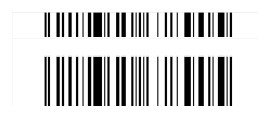
\includegraphics[width=0.5\linewidth]{1Dbarcodes.jpg}
\caption{Cambiar la altura de las barras no cambia la información que contienen}
\label{fig:1dbarcodes}
\end{figure}
\begin{figure} 
\centering
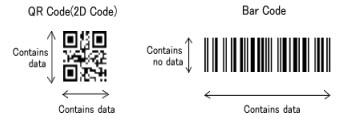
\includegraphics[width=0.5\linewidth]{QRvsBarcode.jpg}
\caption{El código QR (izquierda) contiene información tanto horizontal como vertical, mientras el código de barra (derecha) solo horizontal.}
\label{fig:barcode}
\end{figure}

 % tecnologia anterior al codigo qr

%origen
\section{Origen y Antecedentes}

En 1994, se inventó el sistema de código QR por Masahiro Hara y un asociado de la empresa japonesa Denso Wave.\cite{2019_Hara}
\\
Los códigos QR fueron creados en Denso Wave Incorporated, Japón. Denso Wave es una empresa subsidiaria de Toyota. Se diseñaron con el proposito de gestionar los inventarios de piezas, en las plantas de fabricación de automóviles.  Han decidido no ejercer su derecho de patente para difundir su uso, pero la empresa posee la marca registrada del código.\cite{2014_Chang,2015_Emran_BOOK} 
\\
La empresa introdujo los códigos de barras en el método kanban de Toyota, proponiendo así un sistema de producción integrado para productos e información. ``Kanban'' se basa en la filosofía esencial de Toyota y es una herramienta para realizar el método de producción justo a tiempo. Es una hoja de especificación que se adjunta a una pieza y con ello durante todo su recorrido. Ahora bien, cuando empezó a aumentar el volumen de la producción, se tenían que procesar más hojas de especificaciones y se producían más errores humanos, ya que la entrada de datos se realizaba de manera manual a la computadora. Por esa razón, los códigos de barras se introdujeron en el ``kanban'' junto con escaners de códigos que lograba la entrada de forma automática en la computadora. Comenzó con el desarrollo del código QR en 1992. De hecho, los códigos de barras se usan ampliamente como un método de entrada, preciso, rápido y con un bajo coste en forma impresa.\cite{1998_Institute_Kore}

\begin{figure} 
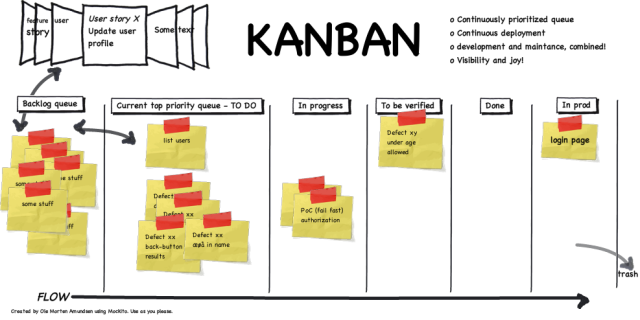
\includegraphics[width=0.6\textwidth]{kanbantoyota.png}
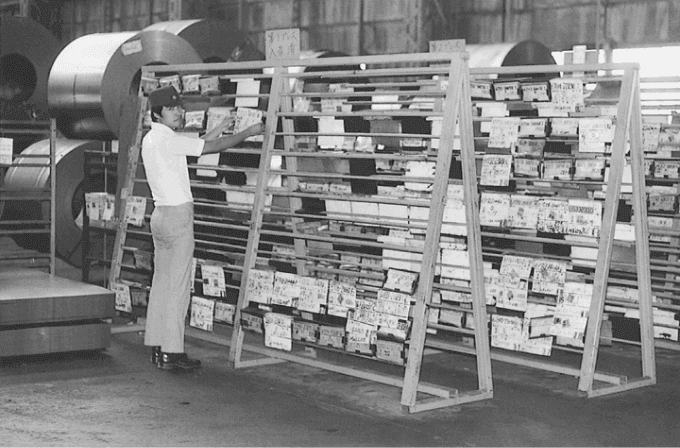
\includegraphics[width=0.4\textwidth]{kanban-board-toyota.png}
\caption{Kanban, cuyo significado es letrero o tarjeta en japonés, es un sistema de información que controla de modo armónico la fabricación de los productos necesarios en la cantidad y tiempo necesarios en cada uno de los procesos que tienen lugar tanto en el interior de la fábrica, como entre distintas empresas.}
\label{fig:kanban1}
\end{figure}

Sin embargo, las tendencias cambiaron de la producción en masa a la producción de ``bajo volumen de productos múltiples''. Para el control de producción finamente ajustado en las plantas de fabricación y, con el aumento del volumen de información manejada, se tuvieron que leer varios códigos de barras diferentes ralentizando la eficiencia de la producción y además de fatigar a los trabajadores. Se puede señalar que tras el colapso de la burbuja económica, muchas empresas buscaron calidad como diferenciación de sus productos. Por tal motivo, se deseaban mantener el control a nivel de componentes, demandando un código que pudiera imprimirse en componentes de tamaño micro como IC.\cite{2002_Hoshino}

 % Origen y razones del desarrollo del codigo qr

%caracteristicas
\section{Características}

\subsection{Alta velocidad de decodificación}
La alta velocidad de decodificación permite minimizar el tiempo de lectura y, también utilizarlos en dispositivos con recursos de computación limitados.\cite{2012_Encinas}

\subsection{Bajo coste del decodificador}
Los códigos bidimensionales QR solo necesitan una cámara de baja resolución para capturar el código y software para procesarla. Es posible, usar télefonos moviles o una webcam. Para el decodificado del código, existen numerosas implementaciones en software de uso libre o código abierto y librerías.\cite{2012_Encinas}

\begin{figure} 
\centering
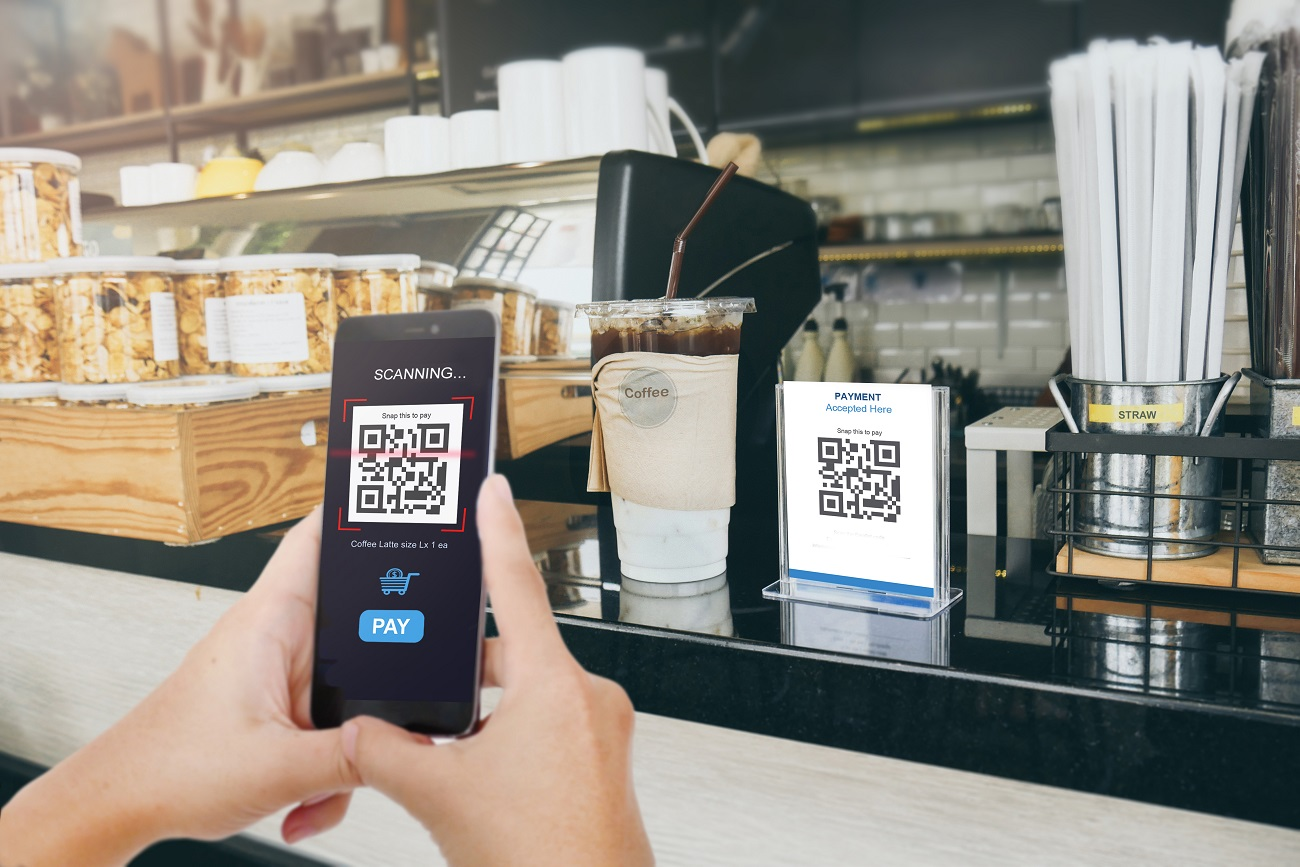
\includegraphics[width=0.4\textwidth]{escanear-codigo-qr.jpg}
\caption{Lectura de los códigos QR, mediante una aplicación.}
\label{fig:costedecodificador}
\end{figure} 

\subsection{Facilidad de lectura}
Un código QR puede ser leído desde cualquier dirección en 360 grados. Esto es posible debido a los patrones de detección de posición en las tres esquinas del símbolo, hacen que el código QR se pueda identificar y leer de forma rápida.\cite{2014_Chang}
Los patrones permiten reorientarlo automáticamente una vez que son capturados por la cámara, eliminando cualquier interferencia de fondo, lo que garantiza una lectura estable de alta velocidad.\cite{2012_Encinas,2012_DENSO}


\subsection{Gran capacidad de codificación de datos}
Los códigos de barras tradicionales solo almacenan hasta 20 dígitos. En cambio, la característica más importante del código QR es la codificación de datos, puede proporcionar hasta 200 veces más información que los códigos de barras unidimensionales. El código QR puede codificar hasta poco más de 7,000 caracteres o 300 caracteres alfanuméricos.\cite{2014_Chang,2012_DENSO} Dependiendo del tipo de dato a codificar la capacidad del código QR varia, siendo superior a la de otros códigos bidimensionales.   Por ejemplo, si los datos son numéricos, el máximo es de 7,089 caracteres; si son alfanuméricos, el máximo es de 4,296 caracteres; en cambio, si son binarios, el máximo es de 2,953 bytes.\cite{2012_Encinas}
%highcapacitydatastorage
\begin{figure} 
\centering
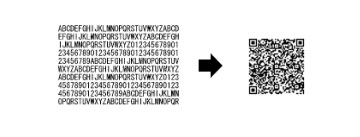
\includegraphics[width=0.7\textwidth]{highcapacitydatastorage.jpg}
\caption{Un código QR de este tamaño puede contener 300 caracteres alfanuméricos.}
\label{fig:datastorage}
\end{figure} 

\subsection{Gran resistencia frente a errores y daños}
El contenido en un código QR es posible recuperarla, aunque parte del mismo tenga errores, este dañada o manchada.\cite{2012_Encinas}
Para recuperar la información, el código QR tiene la capacidad de realizar corrección de errores. La restauración de datos depende de la proporción del daño que tiene el símbolo.\cite{2014_Chang}
%ErrorCorrectionCode.jpg
\begin{figure} 
\centering
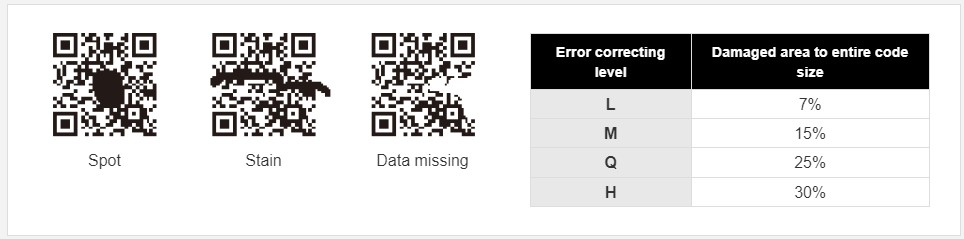
\includegraphics[width=0.9\textwidth]{ErrorCorrectionCode.jpg}
\caption{El código Reed-Solomon se aplica para restaurar los datos cuando una parte del código QR falta o está dañada. La tasa de restauración varía en 4 niveles diferentes de corrección de errores.}
\label{fig:ErrorCorrectionCode}
\end{figure} 

De acuerdo con el nivel de corrección de errores elegido, se puede decodificar hasta un máximo del 30\% de los datos si están sucios o dañados. Un símbolo de código QR se puede leer incluso si su imagen está curvada o distorsionada. \cite{2012_DENSO}
El código Reed-Solomon se desarrolló originalmente como una medida contra el ruido de comunicación para sondas planetarias y para satélites artificiales. Siendo uno de los métodos matemático de corrección de errores usados en los discos compactos de música, es capaz de realizar la corrección a nivel de bytes, y es adecuado para códigos de errores de ráfaga concentrados.\cite{2004_Ohmsha,2008_Conf}
En cambio, si uno o más de los patrones de detección de posición en las tres esquinas del símbolo es borrado o eliminado, no sera capaz de reorientarlo automáticamente, por ende, incapaz de decodificarlo.
\begin{figure} 
\centering
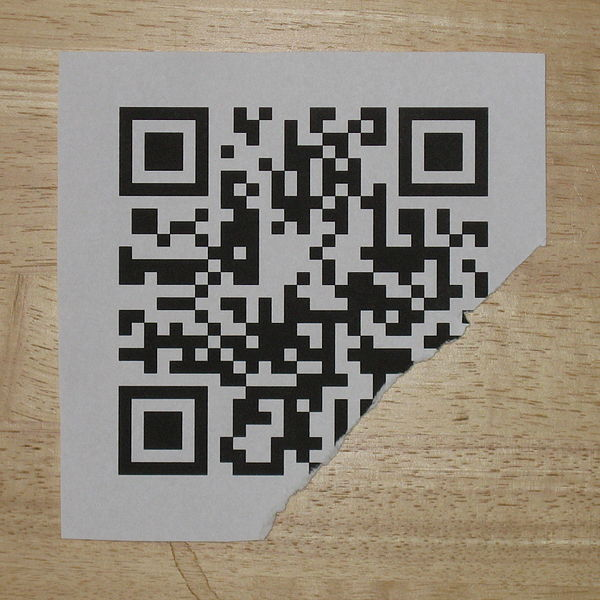
\includegraphics[width=0.3\textwidth]{QR_Code_Damaged.jpg}
\caption{Código QR dañado pero es capaz de decodificarse.}
\label{fig:ErrorCorrectionCode1}
\end{figure} 

\subsection{Posibilidad de personalización}
El símbolo de código QR tiene una estructura bidimensional, se puede usar un código micro QR para un tamaño de impresión más pequeño.
Dado que tiene una gran resistencia frente a errores y daños, los códigos QR se pueden personalizar añadiendoles color, superponiendo algún elemento propio de la imagen de alguna empresa o modificando alguna parte del código.\cite{2014_Chang,2012_Encinas}
\begin{figure} 
\centering
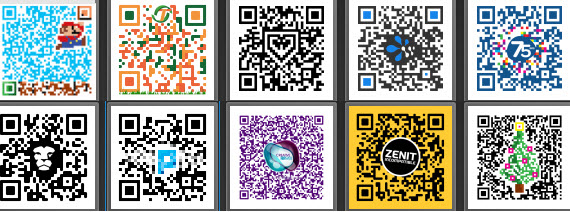
\includegraphics[width=0.7\textwidth]{codigos-qr-creativos-logos.jpg}
\caption{Códigos QR personalizados}
\label{fig:qrpersonalizados}
\end{figure} 


\subsection{Adaptación al tamaño de los datos}
Un código QR puede contener la misma cantidad de datos que un código de barras unidimensional en solo una décima parte del espacio.\cite{2012_DENSO}
Dependiendo de la cantidad de datos a codificar en el símbolo de código QR, el estándar permite utilizar hasta 40 versiones. Cada versión tiene mayor capacidad de codificación que la anterior, a mayor cantidad de datos a codificar; mayor será la versión. Las versiones solo quedan definidas por el número de módulos que se utilizan para su representación. El elemento más pequeño (celda blanca o negra) del código QR se llama ``un módulo''. \cite{2012_Encinas}
\begin{figure} 
\centering
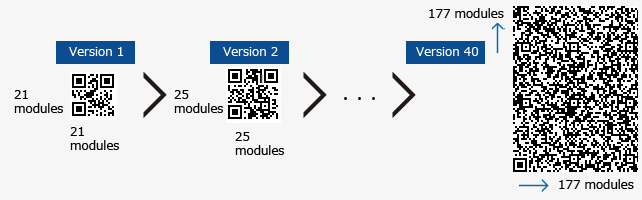
\includegraphics[width=0.7\textwidth]{versionVarietyImage.png}
\caption{Versiones del código QR}
\label{fig:Versiones}
\end{figure} 
Otra característica del código QR es su característica de anexión estructurada. Permitiendo imprimir su estructura en un espacio más reducido. En otras palabras, un símbolo de código QR pueden contener hasta 16 símbolos más pequeños separados, cada uno de los cuales contiene información única. También es posible dividir un solo símbolo de código QR entre cuatro diferentes códigos QR.\cite{2014_Chang}
%qrdivide4.png
\begin{figure} 
\centering
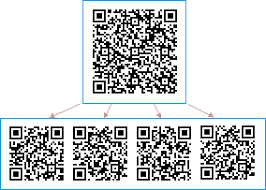
\includegraphics[width=0.5\textwidth]{qrdivide4.png}
\caption{El código QR único se puede dividir en cuatro códigos diferentes.}
\label{fig:qrdivide4}
\end{figure} 

 % Caracteristicas del codigo qr.

%tipos de codigos qr
\section{Tipos de Códigos QR}

\subsection{Código QR Modelos}
\begin{figure} 
	
\includegraphics[width=0.4\linewidth]{model1Image.png}
	
\includegraphics[width=0.4\linewidth]{model2Image.png}
	\label{fig:QRModels}
\end{figure}

\subsubsection{Código QR Modelo 1}
Es el código QR original, es capaz de codificar 1,167 números con una versión máxima de 14 (73 x 73 módulos). \cite{qrcode2021}

\subsubsection{Código QR Modelo 2}
Mejora del modelo 1 para que este código se pueda leer sin problemas incluso si está distorsionado de alguna manera. Por ejemplo, si los códigos QR están impresos en una superficie curva o distorsionada de alguna manera, debido al ángulo de lectura se pueden leer de manera eficiente, utilizando sus patrones de alineación. Estos pueden códificar 7,089 números, siendo su versión máxima de 40 (177 x 177 módulos).\cite{qrcode2021}

\begin{figure} 
	\centering
	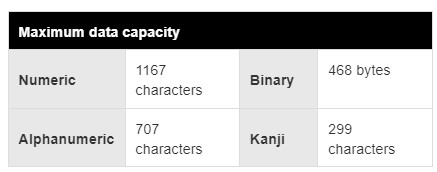
\includegraphics[width=0.7\linewidth]{qrmodel1Maxdata.jpg}
	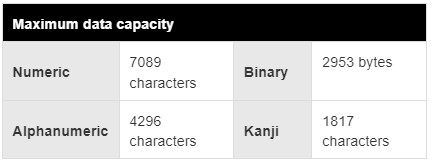
\includegraphics[width=0.7\linewidth]{qrmodel2Maxdata.jpg}
	\caption{Capacidad Máxima de datos del modelo 1 y 2 respectivamente.}
	\label{fig:qrmodel2Maxdata}
\end{figure} 

\subsection{Micro código QR}

En 1998, se desarrolló el micro código QR que mantiene el rendimiento de lectura del código QR, permite la codificación de 20 caracteres alfanuméricos que se incluían en códigos de productos y número de series, siendo impreso en un cuadrado de 1mm.\cite{2019_Hara}
\begin{figure} 
	\centering
	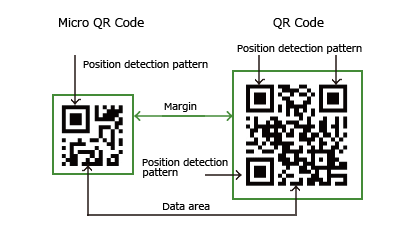
\includegraphics[width=0.4\linewidth]{microQrImage.png}
	\caption{Diferencias entre un código QR y uno micro código QR.}
	\label{fig:microQR}
\end{figure}
El micro código QR se distingue por el hecho de que solo tiene un patrón de detección de posición, en comparación con el código QR que requiere un área, dado que los tres patrones de detección de posición se encuentran en las esquinas del símbolo. Mientras que el micro código QR solo requiere un margen de dos módulos alrededor de un símbolo, donde el Código QR tradicional requiere al menos un margen de cuatro módulos. Esto permite que sea impreso en áreas incluso más pequeñas que el código QR. La cantidad máxima de datos que puede almacenar es de 35 números, con una versión máxima M4 (17 x 17 módulos).\cite{qrcode2021}



\subsection{Código iQR}
El código iQR es un código bidimensional que permite una fácil lectura de su posición y tamaño. Tiene una amplia gama de códigos de tamaño, puede contener una mayor cantidad de datos que el código QR tradicional, con el mismo tamaño se puede contener un 80\% más que este último. Además, el código iQR es de 9 x 9 módulos con eso se puede reducir un 30\% más pequeño en relación a el código QR que consta de 11 x 11 módulos. Este código se puede imprimir como un código rectangular, un código invertido, inversion de los colores de los módulos o un código de patrón de puntos (marcado directo de piezas). Debido a esto, es posible colocarlos en una superficie cilíndricas manteniendo su legibilidad del código, lo que no es posible con códigos cuadrados.\cite{qrcode2021}
\begin{figure} 
	\centering
	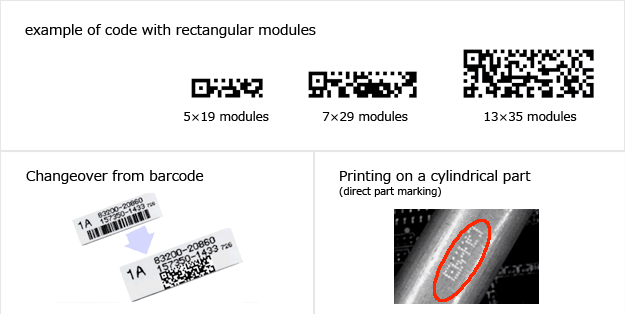
\includegraphics[width=0.8\linewidth]{iQrFeature3Image.png}
	\label{fig:iqr}
\end{figure}
\begin{figure} 
	\centering
	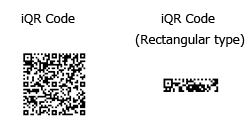
\includegraphics[width=0.4\linewidth]{iQrCodeImage.png}
	\caption{Código Cuadrado y Código Rectangular, respectivamente.}
	\label{fig:iqr2}
\end{figure}

Por otro lado, el número de caracteres que puede almacenar el código iQR es de 40,000 caracteres numéricos en su versión más grande (422 x 422 módulos). En donde su nivel de corrección de errores es de hasta el 50 \%. Su forma rectangular, el mínimo es de 5x19 puede almacenar 6 números y el de módulo máximo es de 43 x 131, aproximadamente 1,200 caracteres.\cite{qrcode2021}
El código iQR rectangular con mayor eficiencia de datos fue desarrollado en 2008.\cite{2019_Hara}

\subsection{Código SQRC}
Utilizando la tecnología Secure QR Code (SQRC) para mantener la información segura y oculta. Debe señalarse que para compartir la información personal confidencial es necesario la validación y autorización del código QR mediante el algoritmo criptográfico de clave pública RSA.\cite{Ahamed2019}
La estructura del código SQRC cuenta con dos capas, una región de información abierta y una región de información cerrada. La región abierta puede ser leída por cualquier dispositivo con capacidad de escaneo, mientras que la region cerrada encryptada que solo se puede leer con dispositivos que cuenten con las claves de cifrado coincidentes y un software especial de reconocimiento (para verificar que los datos no sufrieron alteraciones).\cite{2019_Hara}
\begin{figure} 
	\centering
	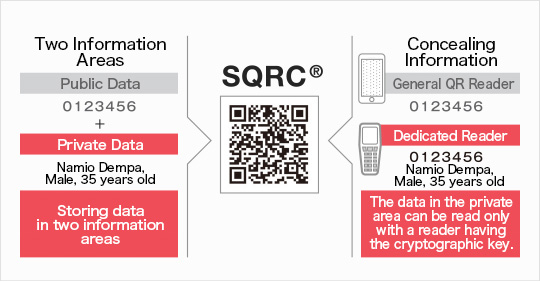
\includegraphics[width=0.4\linewidth]{SQRC.jpg}
	\caption{Utilizando una clave criptográfica para mantener la información privada y con esto restringir los tipos de dispositivos que pueden leer la información.}
\label{fig:sqrc}
\end{figure} 

El código SQRC puede evitar la falsificación y manipulación. El código QR aunque tiene mayor espacio y gran capacidad, se puede leer la información con cualquier dispositivo, incluida la información privada y clasificada, por esta razón no es seguro. El uso de este código puede darse en Hospitales (protección y gestión de información personal), Delivery de albaránes entre empresas, instalaciones de eventos y parques de atraciones.\cite{qrcode2021}

\subsection{Código Frame QR}
Frame QR es un código con la misma capacidad que el código QR original, pero establece un lienzo especial que contiene algún logotipo o imagen en el centro del código. \cite{2019_Hara}
\begin{figure} 
	\centering
	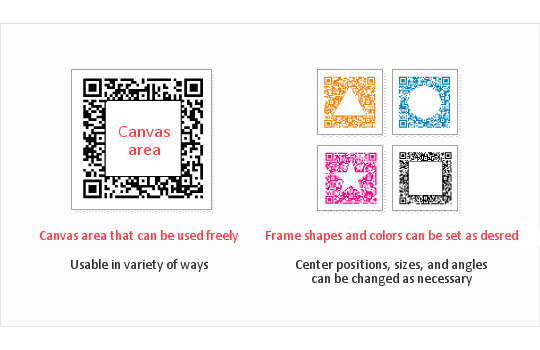
\includegraphics[width=0.6\linewidth]{FrameQR.jpg}
	\caption{Tiene un área que puede contener un tipo de forma, logotipo o imagen dentro de ella.}
	\label{fig:frameqr}
\end{figure}
Este código tiene un marco para contener una imagen. Tanto la forma del marco y el color se pueden cambiar, se puede aplicar a una variedad de aplicaciones. El uso de este código puede darse en Tarjetas de visita y catálogos, Medidas anti-falsificación y trazabilidad.\cite{qrcode2021} %Tipos del codigo qr.

%variantes

\section{Variantes}

\subsection{Portable Data File - PDF417}
El código de barras bidimensional PDF417 (Archivo de datos portátil), es el más utilizado y el más antiguos. El código de barras apilado está compuesto por filas de códigos de barras lineales. Siendo bidimensional, le permite llevar más información que los códigos unidimensionales. La razón del número 417, es porque cada patrón o palabra de código codificada en el código de barras está representada por cuatro barras y cuatro espacios. Donde el ancho total de cada palabra de código es de 17 módulos de ancho.
\\
El código de PDF417 empaqueta más información y proporciona redundancia adicional mediante el uso de la técnica de corrección de errores Reed Solomon. Por tal motivo, necesitarán más áreas del código de barras; algunas partes de esa área se utilizarán para la corrección de errores y dará como resultado que se codifiquen menos información. Además, admite diferentes modos de compactación permitiendo que, diferentes tipos de datos sean codificados de manera óptima en el símbolo, por ejemplo, el modo de compactación alfanumérica extendida (EXC) admitiendo la codificación de todos los caracteres ASCII imprimibibles y comprimirlos 2 caracteres por palabra de código.\cite{PDF417Barcode2021}
%496px-PDF417_Example.png
\begin{figure} 
	\centering
	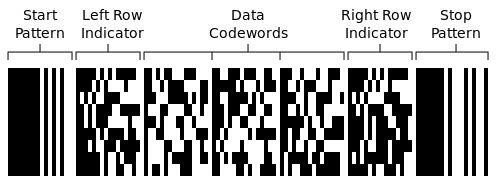
\includegraphics[width=0.7\linewidth]{496px-PDF417_Example.png}
	\caption{Partes de un código o símbolo PDF417. Son omitidas las zonas tranquilas del código.}
	\label{fig:pdf417example}
\end{figure} 

El código PDF417, del desarrollador Symbol Technologies tiene un formato de código de barras apilado. La capacidad de datos varia dependiendo del tipo de datos, para casos númericos 2,710; para alfanúmericos 1,850; binario 1,018 y Kanji 554. Su característica principal es su gran capacidad y sus aplicaciones principales son la automatización de oficinas, licencias de conducir,y también se puede utilizar en los medidores de correo para codificar la cantidad de franqeo, así como en los paquetes de FedEx.\cite{2012_DENSO,2004_FedEx_TECH_REPORT}

\begin{figure} 
	\centering
	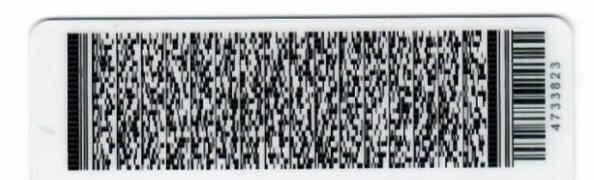
\includegraphics[width=0.7\linewidth]{cedulapdf417.jpg}
	\caption{PDF417 usado en la cédula de identidad (reverso).}
	\label{fig:pdf417CI}
\end{figure} 
\textbf{Ventajas}: Puede codificar cualquier carácter ASCII. Apilar tantos códigos uno encima del otro como desee, permitiendo codificar ilimitada cantidad de datos. Además, para evitar errores, incluye un dígito de control en cada código de barras individual.\cite{cognex.com2021}
\\
\textbf{Desventajas}: Como es posible codificar tanta información como desee en varios códigos apilados, en consecuencia el símbolo crecera de manera proporcional a la cantidad de datos ha codificar.\cite{cognex.com2021}

\subsection{Maxicode}

Maxi Code es un código bidimensional, similar al código unidimensional, pero usa puntos en lugar de barras, con un área de una pulgada al cuadrado, con una diana en el medio, alrededor de ella hay una serie de puntos hexagonaless. También incluye un código de corrección de errores, para que el código se pueda leer incluso si tiene errores o está dañada. Además, de tener varios campos, en los que se codifica el código postal, código de país y código de servicio. También conocido como código Bird's Eye o código UPS.\cite{cognex.com2021}

\begin{figure} 
	\centering
	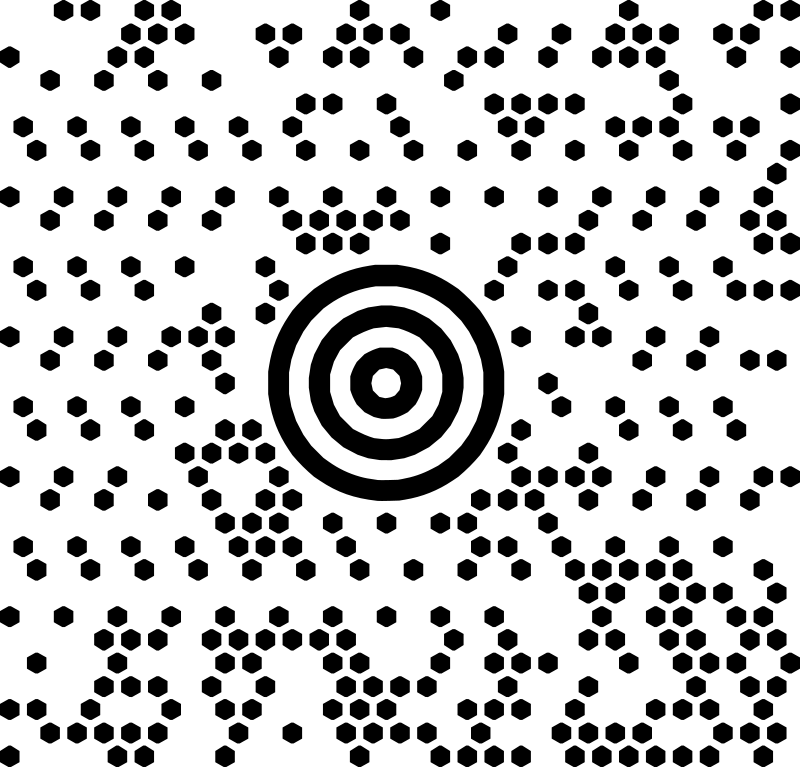
\includegraphics[width=0.2\linewidth]{800px-MaxiCode.svg.png}
	\caption{Ejemplo de un código Maxi.}
	\label{fig:maxicode}
\end{figure} 

El código Maxi, del desarrollador UPS, tiene un formato similar al código QR. La capacidad de datos varia dependiendo del tipo de datos, para casos númericos 138; para alfanúmericos 93; no tiene soporte para tipos de datos binarios y de tipo kanji. Su característica principal es su gran velocidad de lectura y sus aplicaciones principales es en la logística. Se desarrolló originalmente para que lo usara UPS en el seguimiento y envío de paquetes, ya que se puede escanear rápidamente en una cinta transportadora.\cite{2012_DENSO}
\\
\textbf{Ventajas}: escaneo preciso y de forma rápida, incluso en una cinta transportadora en movimiento. \cite{cognex.com2021}
\\
\textbf{Desventajas}: no puede codificar grandes cantidades de información.\cite{cognex.com2021}

\subsection{Datamatrix}

\begin{figure} 
	\centering
	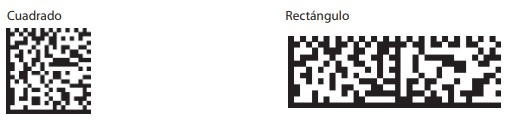
\includegraphics[width=0.5\linewidth]{datamatrix.jpg}
	\caption{Ejemplo de un DataMatrix.}
	\label{fig:DataMatrixRectNormal}
\end{figure}
El código DataMatrix o Matriz de datos, es un código bidimensional, puede tener una configuración cuadrada o rectangular. 
El ECC200 utiliza Reed-Solomon mejorado para la correción de errores eliminado los problemas de distorción, que restaura datos de partes dañadas del símbolo. La tasa de corrección de errores se determina de forma automática dependiendo de la cantidad de datos y el tamaño del símbolo. ECC200 está estandarizado internacionalmente (ISO).\cite{2006_Semacode_TECH_REPORT}

\begin{figure} 
	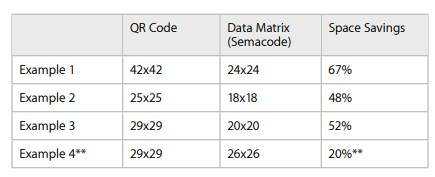
\includegraphics[width=0.6\linewidth]{QRvsDatamatrix.jpg}
	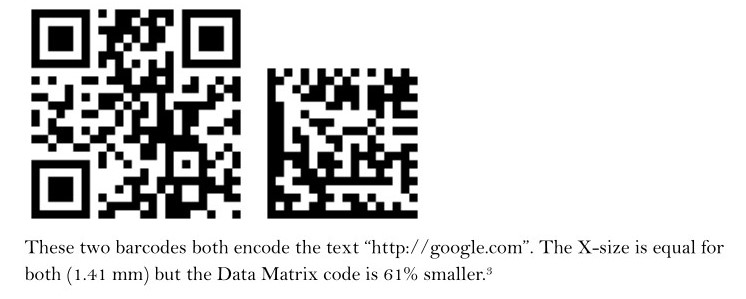
\includegraphics[width=0.6\linewidth]{qrvsdatamatrix2.jpg}
	\caption{Diferencia de espacio entre un código QR y una matriz de datos.(** Caracteres japoneses)}
	\label{fig:datamatrixvsqr}
\end{figure}
En 1989, fue diseñado y estandarizado por socios como la NASA, EE.UU, DoD (U.S. Department of Defense), FDA (Food and Drug Administration) y las industrias como la electronica y el mercado postal. En cambio, QR fue desarrollado en 1994, y su característica distintiva, codificar los caracteres kana japoneses (Kanji).\cite{2006_Semacode_TECH_REPORT}
Pero debido a su pequeño tamaño, existe la dificultad de lectura dado por el enfoque del lector. Por está razón, queda relegado a uso industrial con lectores o escaners especializados. 
\\
El código de matriz de datos, del desarrollador RVSI ACuity CiMatrix, tiene un formato de tipo matricial. La capacidad de datos varia dependiendo del tipo de datos, para casos númericos 3,116; para alfanúmericos 2,355; binario 1,556. Su caraterística principal es su tamaño pequeño y sus aplicaciones principales son la automatización industrial, fabricación de almacenaje, sector sanitario. \cite{2012_DENSO}
\begin{figure} 
%\centering
	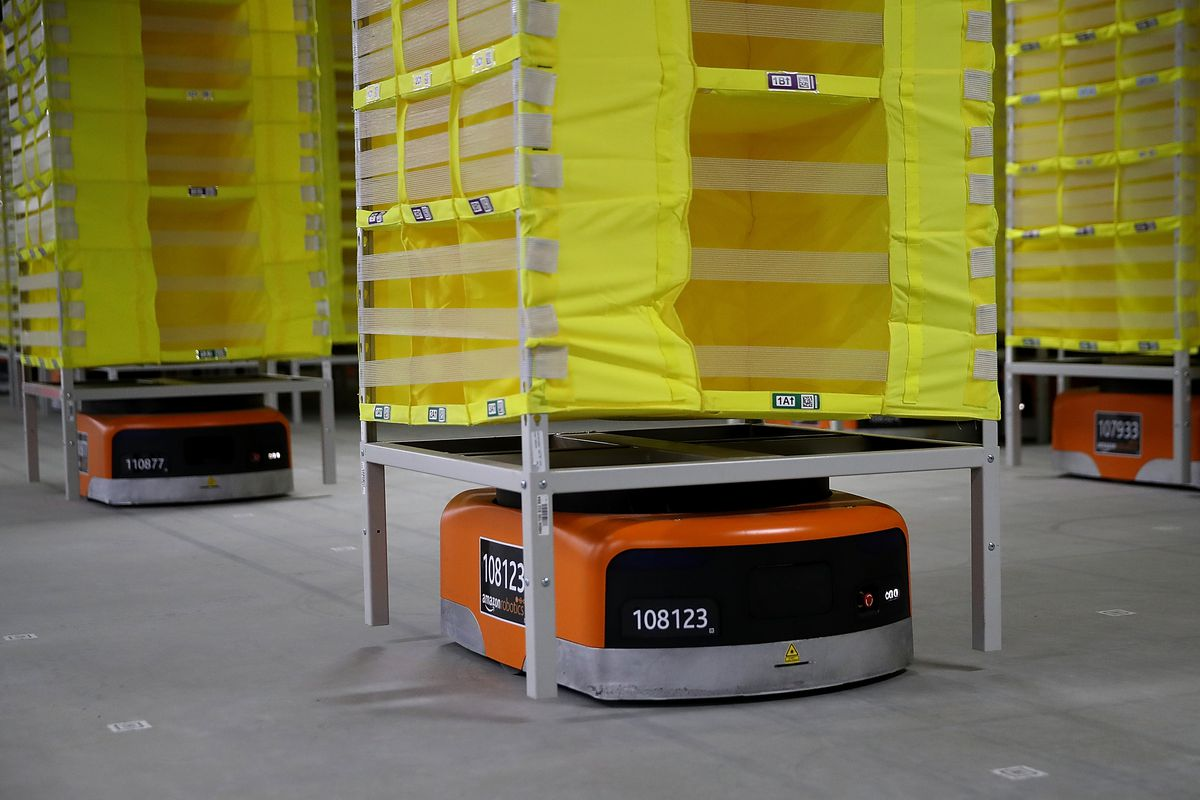
\includegraphics[width=0.5\linewidth]{829377014.jpg.0.jpg}
	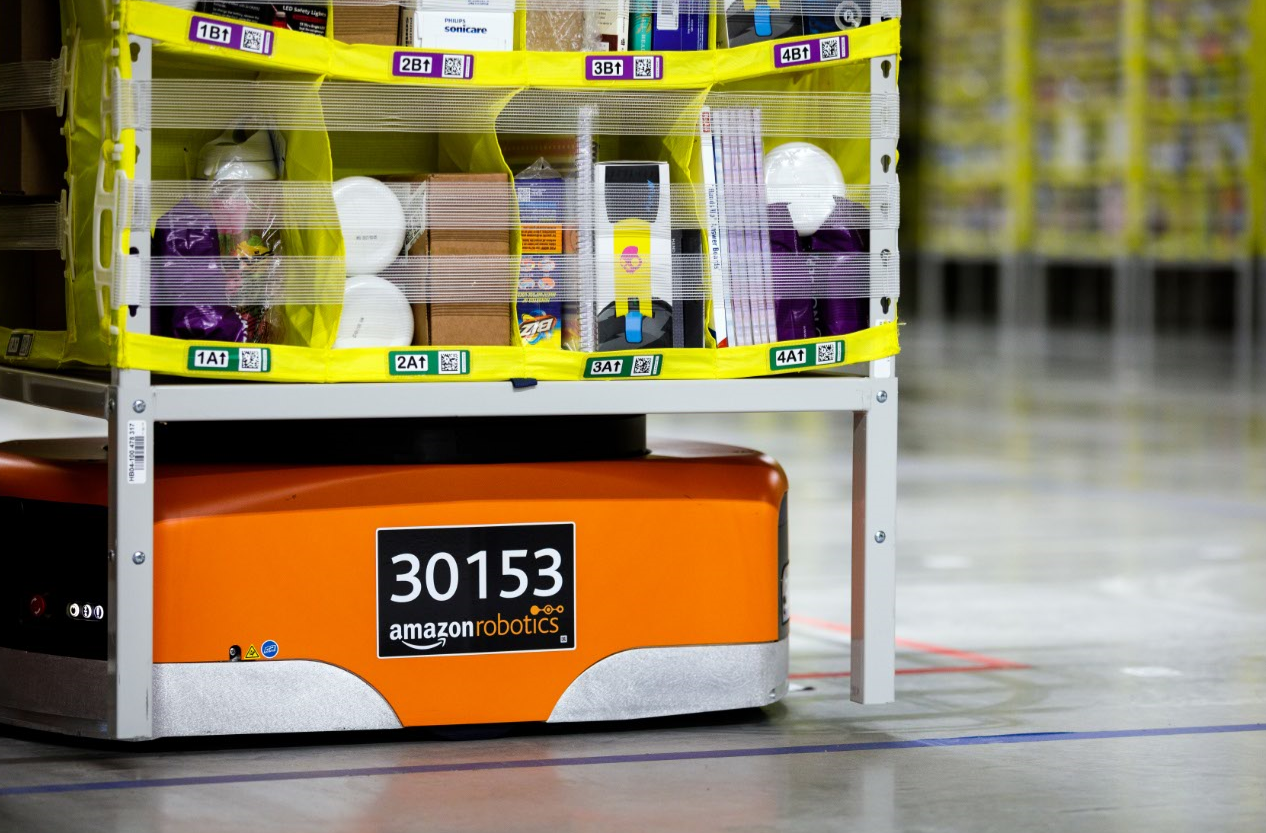
\includegraphics[width=0.5\linewidth]{amazon-robot.png}
	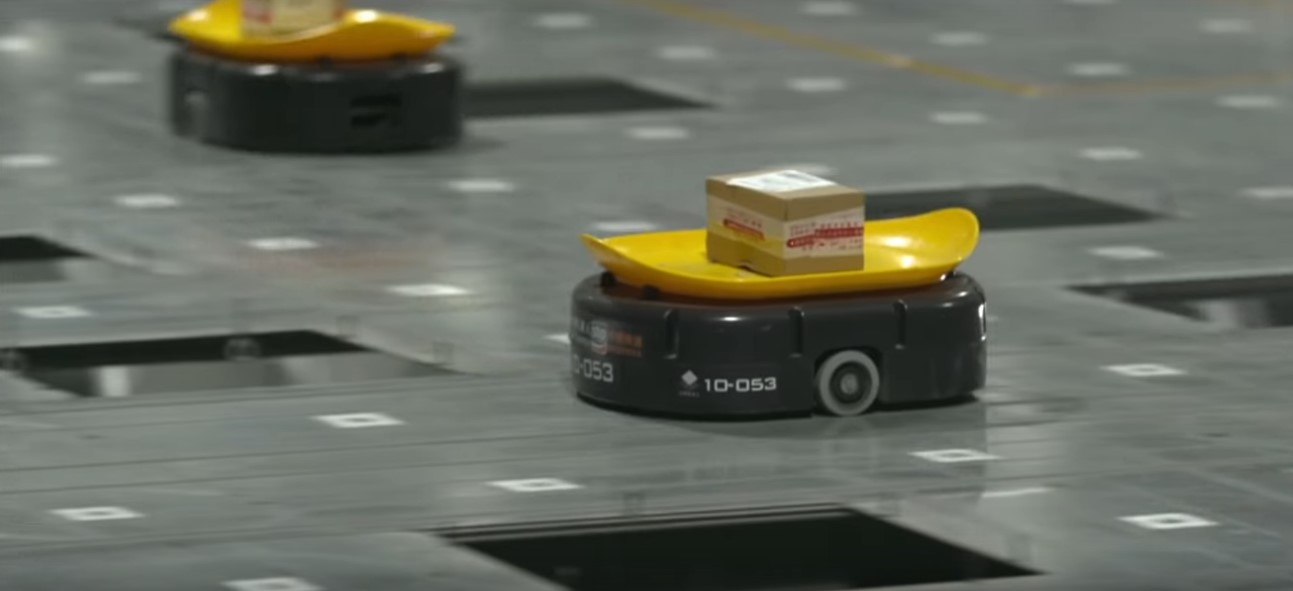
\includegraphics[width=0.5\linewidth]{robotQR.jpg}
	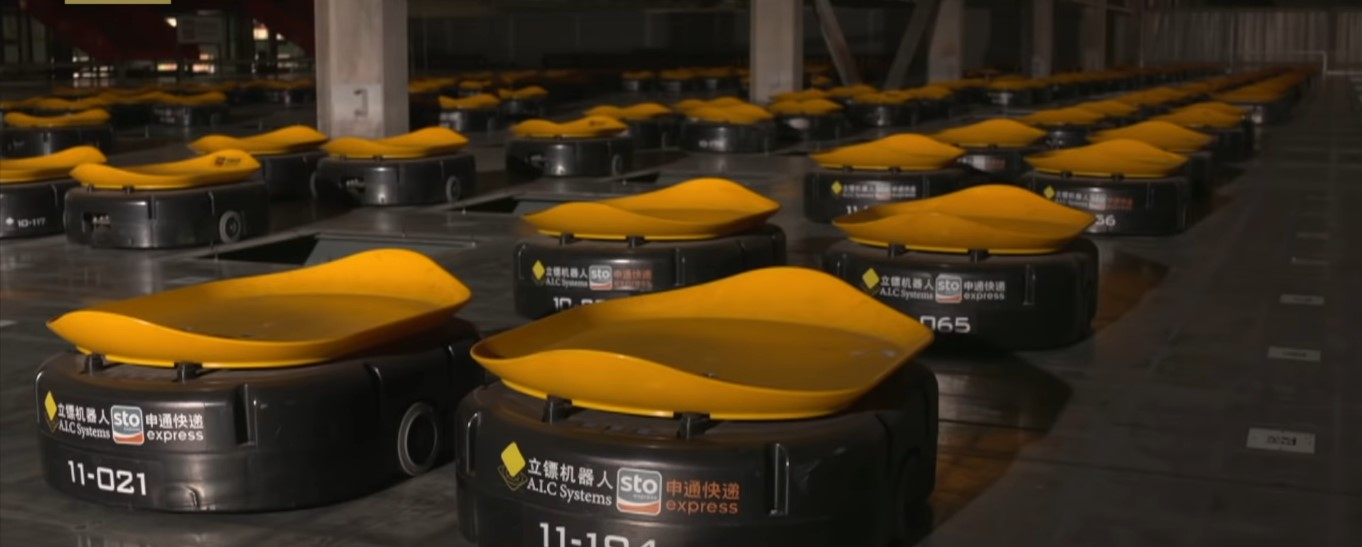
\includegraphics[width=0.5\linewidth]{qrRobot.jpg}
	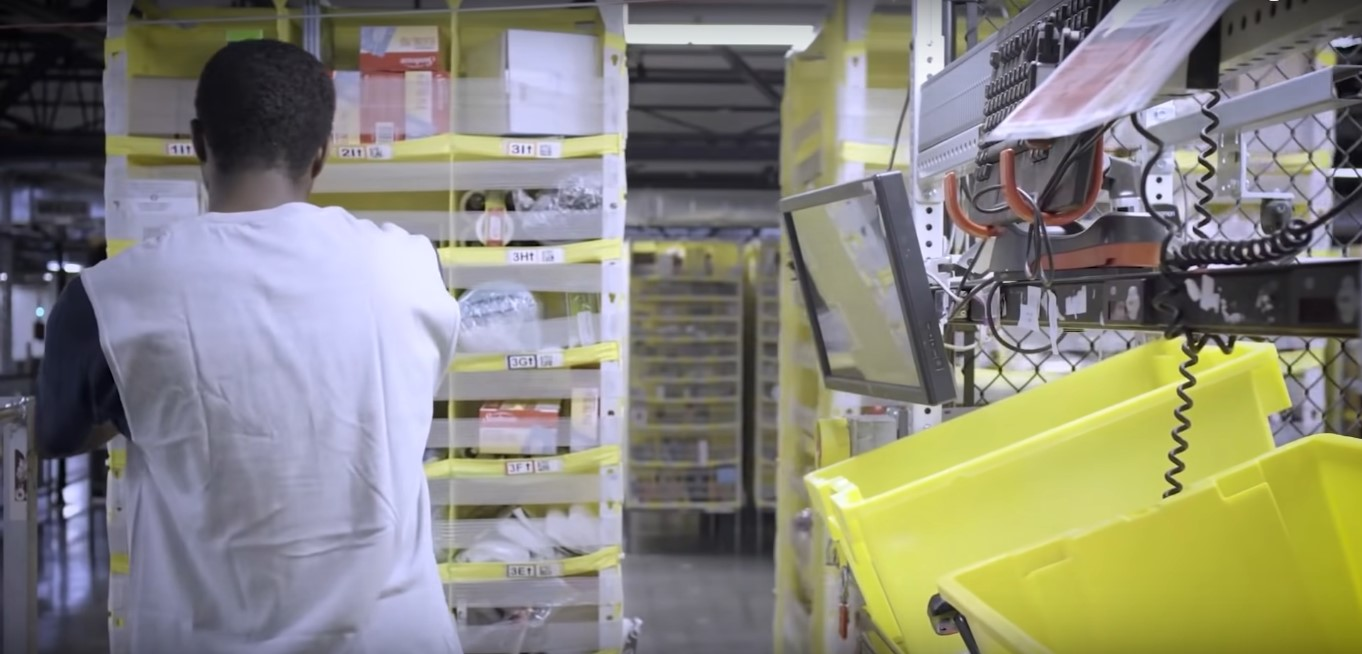
\includegraphics[width=0.5\linewidth]{AmazonSmartWarehouse.jpg}
	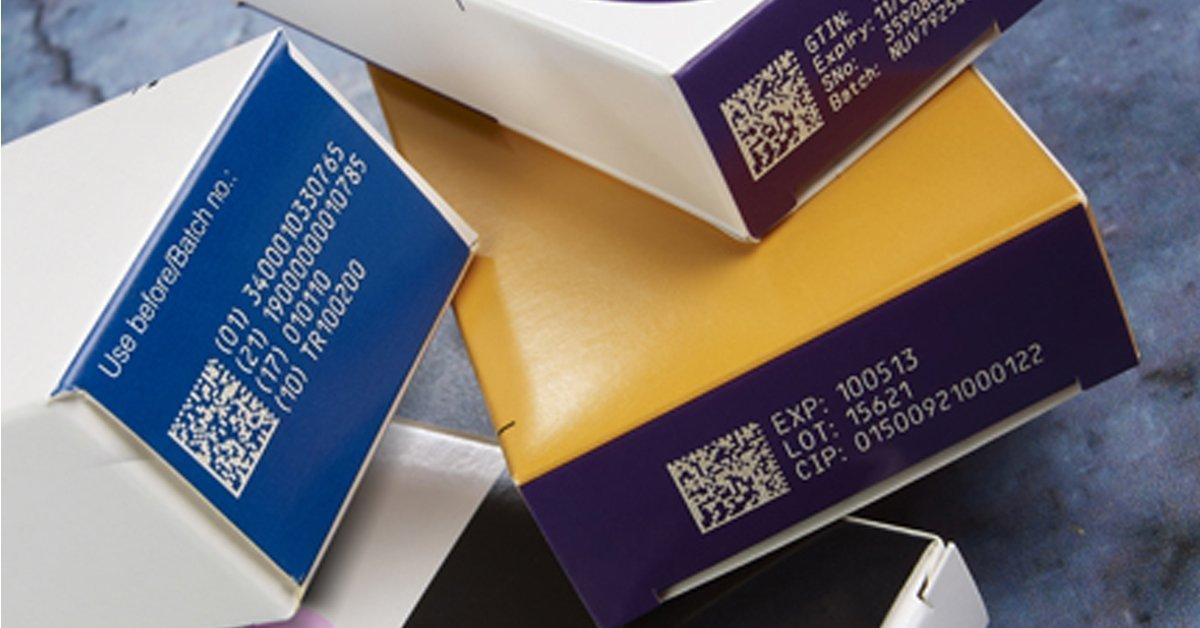
\includegraphics[width=0.5\linewidth]{medicinadatamatrix.jpg}
	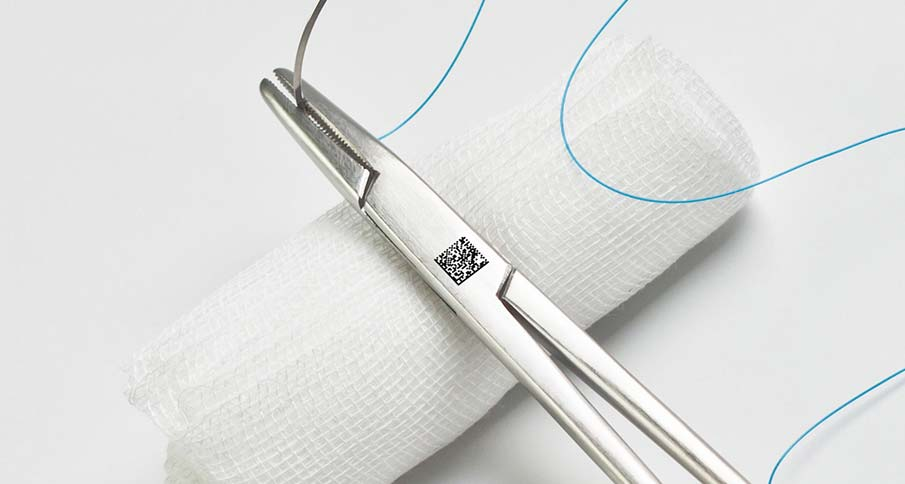
\includegraphics[width=0.5\linewidth]{datamatrixherramientas.jpg}
	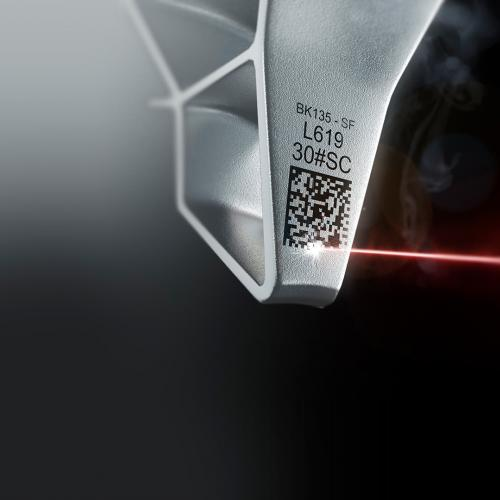
\includegraphics[width=0.3\linewidth]{banner-mkt-a-laser-datamatrix-3d.jpg}
	\caption{Ejemplo de Usos del DataMatrix.}
	\label{fig:datamatrixaplicaciones}
\end{figure}
\newpage
\textbf{“Data Matrix has proven to be the most space efficient of all the twodimensional symbologies.”}
- Consumer Electronics Association’s R9 Automatic Data Capture group (Comparando QR con DataMatrix)\cite{2006_Semacode_TECH_REPORT}
\\
Vea la figura (\ref{fig:datamatrixaplicaciones}), se incluye algunas aplicaciones del código datamatrix, uno de ellos es el uso en los medicamentos o en instrumentos de cirugías por su tamaño y en otros para identificar auto partes (mediante el grabado en metal). En cambio, es también utilizado para automatizar la entrega de los productos, el código es colocado en el suelo; donde los robots se mueven ubicando su posición mediante la lectura del símbolo, complementando con el uso de la tecnología RFID, una vez obtenido se lleva al área de recolección del producto (indicando la cantidad de productos dentro de la pila), donde un trabajador realiza la recolección. Con esto disminuye el espacio del despósito.
\begin{figure} 
	\centering
	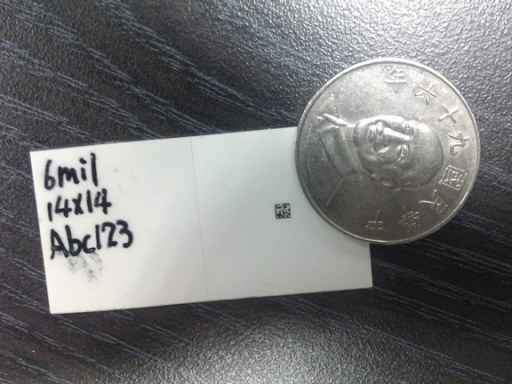
\includegraphics[width=0.4\linewidth]{smalldatamatrix.jpg}
	\caption{Comparando el tamaño de un datamatrix con una moneda.}
	\label{fig:datamatrixmoneda}
\end{figure}

El código Data Matrix utiliza entre un 30\% y un 60\% menos espacio que el código QR conteniendo los mismos datos. El tamaño mínimo es de 10x10 módulos, comparando el mínimo para el código QR es de 21x21 módulos. \cite{2006_Semacode_TECH_REPORT}
\\
El código GS1 DataMatrix, está basado en el estandar ECC200  por GS1 para su distribución y define reglas para diferenciarse del datamatrix tradicional. Se estandarizará en la industria médica, dado que deben imprimirse directamente en instrumentos médicos de acero, como cuchillos quirúrgicos y tijeras. En la versión ECC200, la cantidad de filas y columnas es siempre un número par. El máximo es de 144 filas y 144 columnas divididas en 36 regiones de datos de 22 filas y 22 columnas cada una. En cambio, el formato rectangular, la capacidad máxima es: 72 caracteres alfanuméricos, 98 números. \cite{GS12011}
 % Variantes del codigo QR.

%aplicaciones

\section{Usos y Aplicaciones}

\subsection{Medicina}
% Razón de la elección.
Se diseño y aplicó una pegatina a el yeso de los pacientes de una clínica de fracturas. La etiqueta tenía un código QR, como herramientas de información y de contacto directo al elenco de la clínica para pedir ayuda o consejos. Al retirar el yeso, la gran mayoría tenía la etiqueta; los pacientes completaron un cuestionario sobre la pegatina. La gran mayoría de los pacientes, lo consideraban útil para el manejo proactivo de posibles problemas de yeso.  Otras ramas de la medicina pueden beneficiarse de la incorporación de códigos QR como fuentes de acceso a infomación.\cite{2017_Gough}
\begin{figure} 
	\centering
	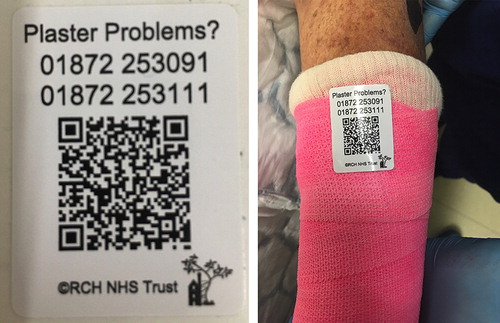
\includegraphics[width=0.5\linewidth]{rcsann.2017.0070-1.jpg}
	\caption{Código QR con fuente de información.}
	\label{fig:qryeso}
\end{figure} 
\\
COVID-19, causado por el SARS-CoV-2, se informaron oficialmente los primeros casos en diciembre de 2019; ha sido declarada pandemia mundial por la Organización Mundial de la Salud (OMS). \cite{2020_Organization} 

Para contener la propagación de enfermedades como el COVID-19, se ha empleado una variedad de enfoques de salud digital.\cite{2020_Breeher}
Uno de ellos, los códigos de salud QR basados en síntomas emitidos por las autoridades de salud pública, son cruciales porque los códigos no recuperan datos de ubicaciones. Los códigos QR se consideran oficialmente certificados electrónicos del estado de salud de las personas,y un certificado más que permitirá la entrada a otro país al dejar constancia que esa persona ha sido vacunada, siendo una medida de movilidad interna; recibiendo el nombre de pasaporte de vacunación o certificado verde digital.\cite{2020_Nakamoto,Commission2021}
\begin{figure} 
	\centering
	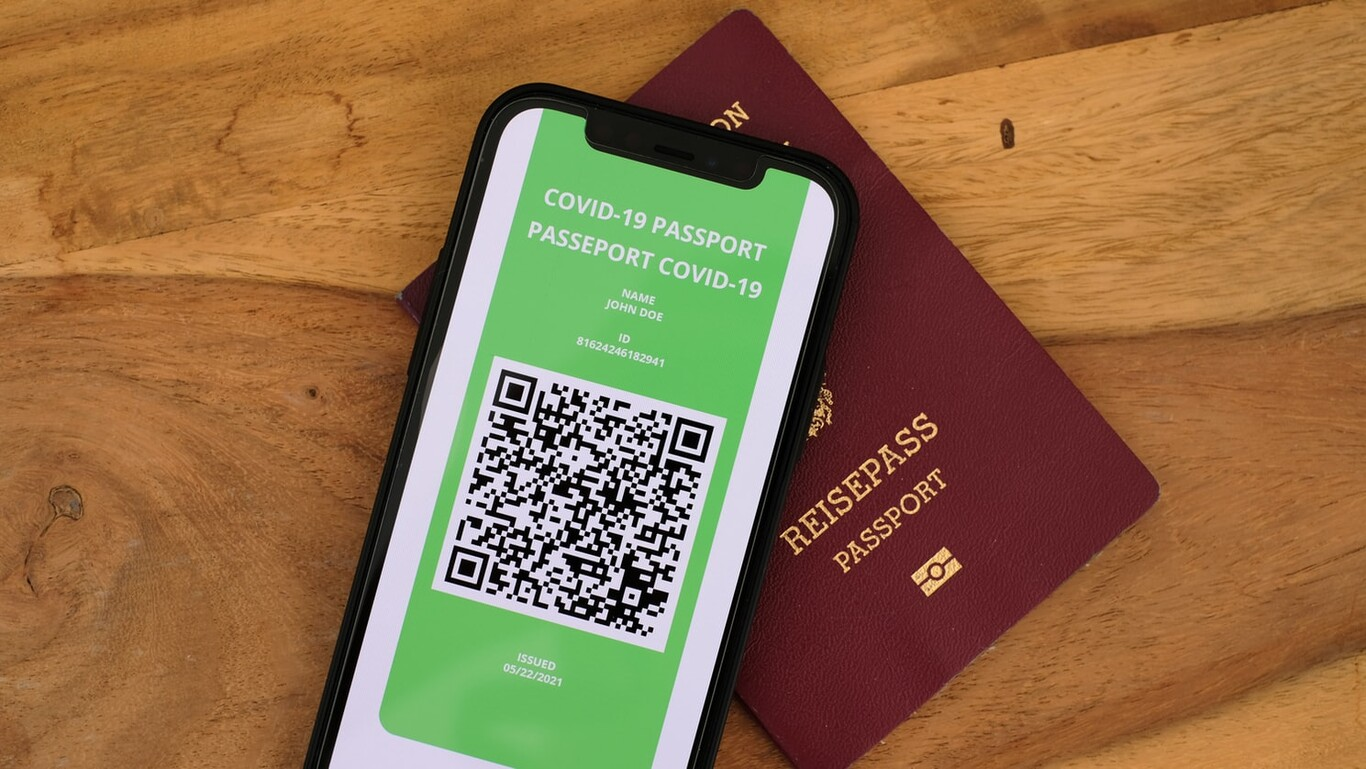
\includegraphics[width=0.5\linewidth]{qrpasaporte2.jpg}
	\caption{Código QR como pasaporte de movilidad.}
	\label{fig:qrpasaporte}
\end{figure} 


\subsection{Marketing y publicidad}
En el medio publicitario, las empresas ofrecen a los consumidores una forma de obtener información relevante de algún producto, ver opiniones de los clientes, ofrecer algún tipo de promoción; una vez que escanean el símbolo puesto en algún anuncio. Motivando el entretenimiento a lo largo de la experiencia, donde los consumidores están más involucrados con las ofertas promocionales; son especialmente importantes para los especialistas en marketing. \cite{2014_Ertekin}
\begin{figure} 
	\centering
	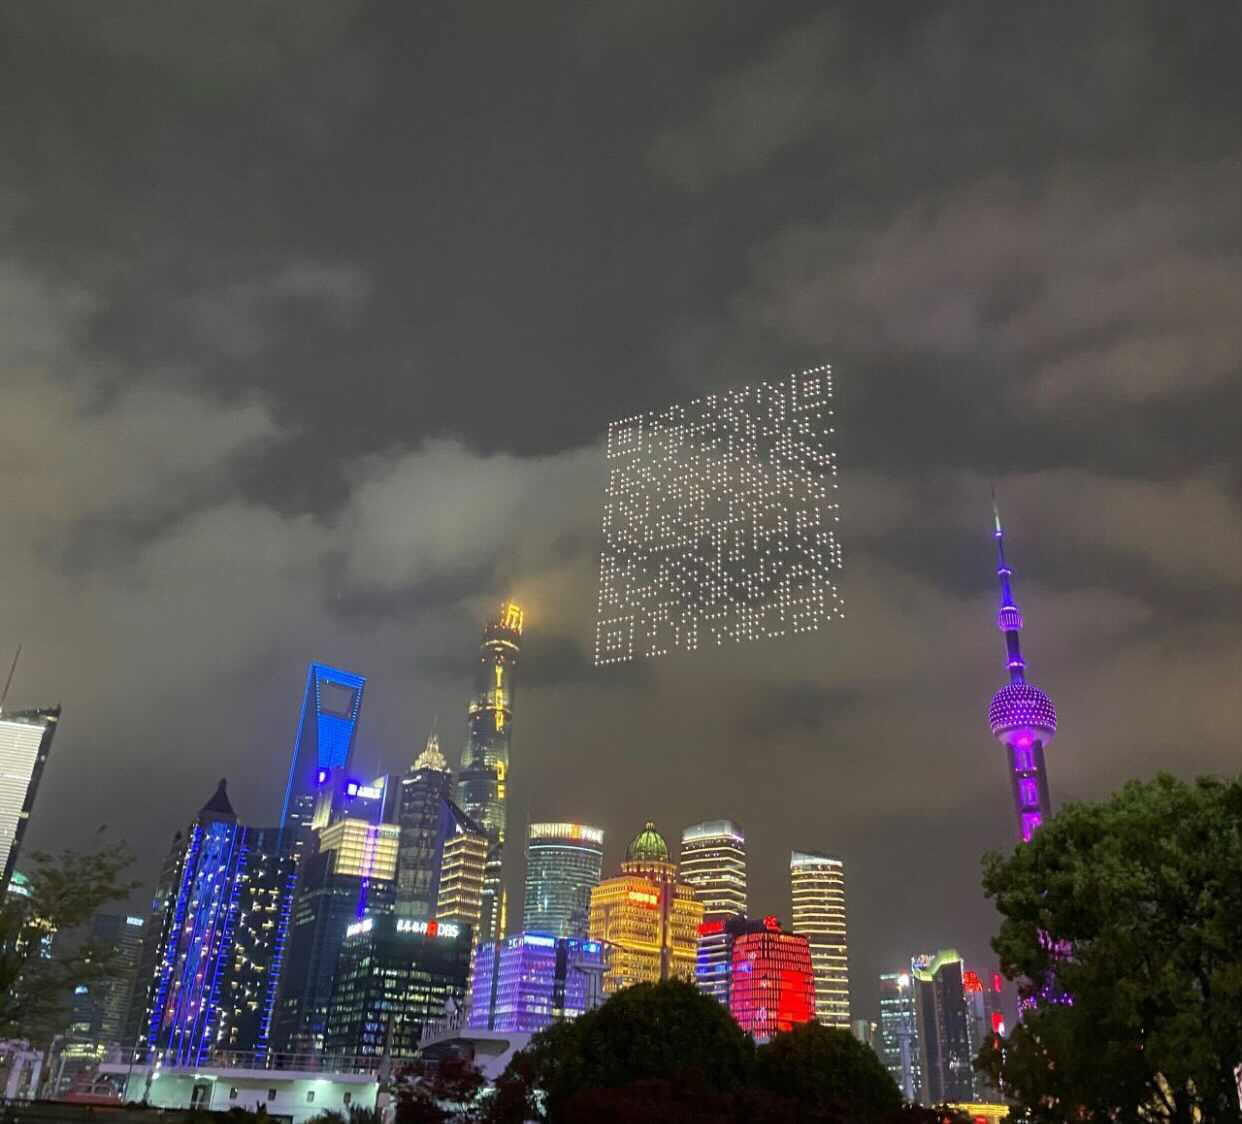
\includegraphics[width=0.5\linewidth]{qrmarketing.jpg}
	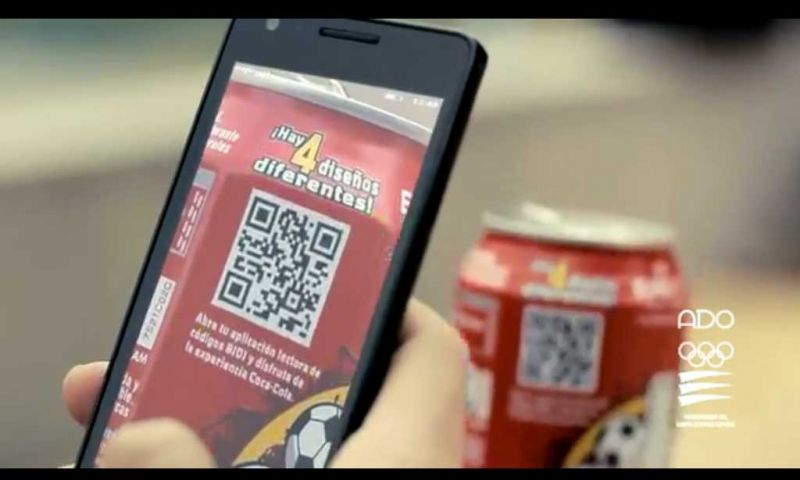
\includegraphics[width=0.5\linewidth]{anuncio-de-coca-cola-uefa-euro-2012-1.jpg}
	\caption{Código QR en Marketing}
	\label{fig:qrmarketing}
\end{figure}
\\
La empresa de bebidas Coca-Cola, fue uno de los primeros en usar los códigos QR en latas. El objetivo no era solo obtener información, busco conectar a los consumidores mediante el escaneo del símbolo, donde estos les redirigia a una página web , donde podían ver vídeos o descubrir conciertos organizados por la empresa. Siendo una buena idea de marketing orientada para los jovenes, lo que mostró el potencial de vincular lo digital con lo real.\cite{Generator2021}
Por lo tanto, pueden considerar tener juegos u otros instrumentos como incentivo para entrener a los consumidores, mediante el escaneo del código QR en anuncios. Llegando a la conclusión, de que son un sustituto factible de los cupones impresos, promociones, navegación entre pantallas y visitas físicas para investigar y obtener detalles del producto. \cite{2014_Ertekin}

\subsection{Entretenimiento}
Los museos y las galerías de arte, utilizan los códigos QR como una forma de experiencia multimedia para sus visitantes, escaneando el símbolo se puede tener una información detallada de las obras de arte, incluso videos, imágenes, audios o una combinación de ambos. Las visitas guiadas se convierten en una experiencia más interactiva, algunas galerías utilizan diferentes técnicas de presentación para atraer más visitantes. Por ejemplo, una empresa australiana, Grande Exhibitions, creó Van Gogh Alive experiencias  y el Museo de Brooklyn ha llevado el uso del código QR para la información del artista, una forma de mejorar la información sobre accesibilidad y también para mostrar el mapa del museo.\cite{2012_Emek}
\begin{figure}
	\centering 
	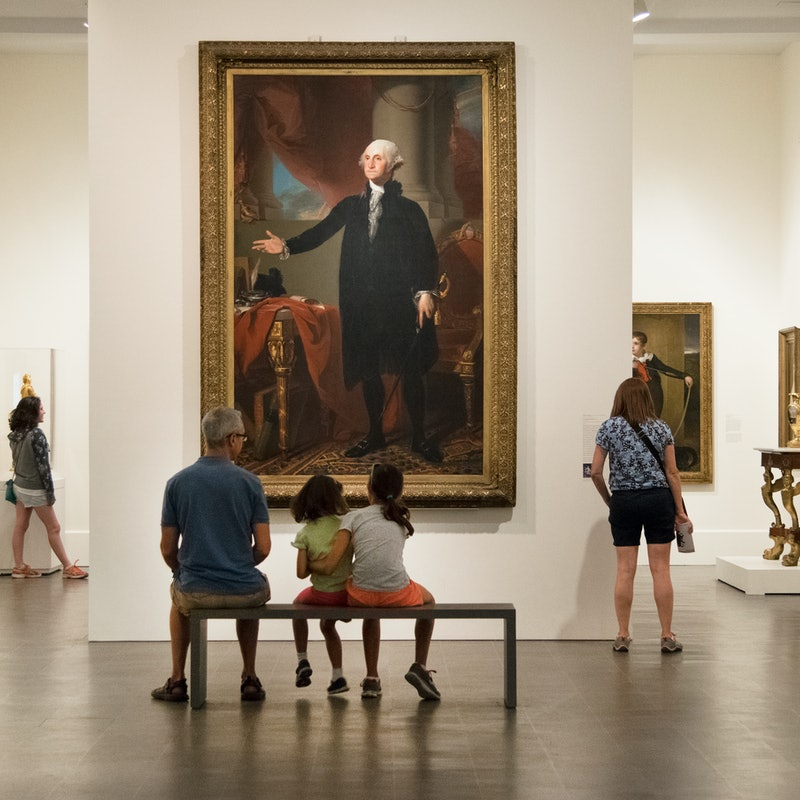
\includegraphics[width=0.4\linewidth]{museobrooklyn.jpg}
	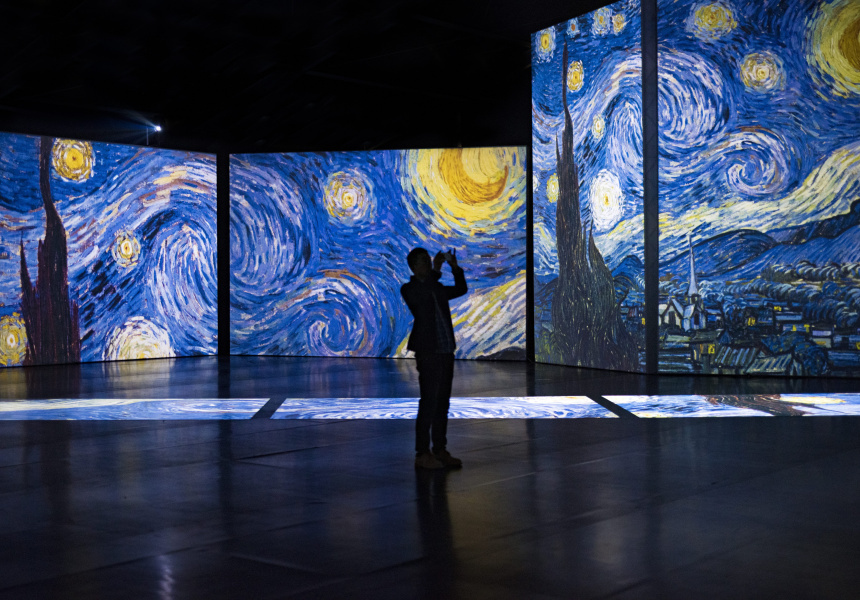
\includegraphics[width=0.4\linewidth]{vangoghalive.jpg}
	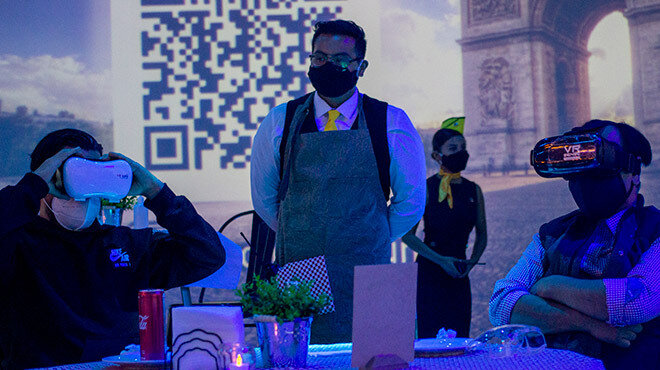
\includegraphics[width=0.4\linewidth]{vangoghalive2.jpg}
	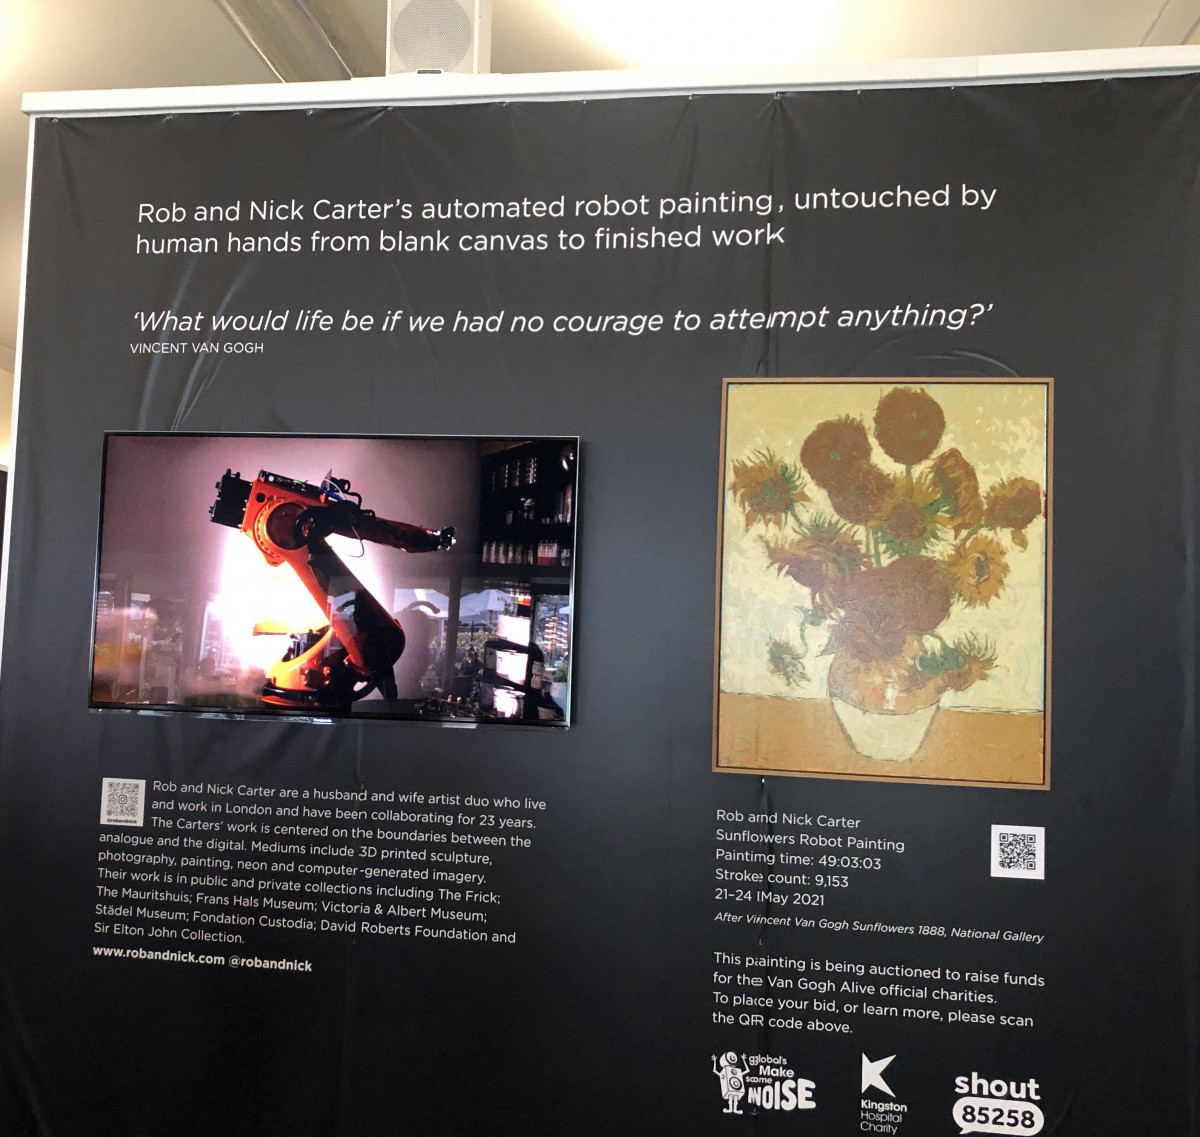
\includegraphics[width=0.4\linewidth]{vangoghalive3.jpg}
	\caption{El código QR en el entretenimiento.}
	\label{fig:qrentretenimiento}
\end{figure}

\subsection{Turismo y Transporte}

La aerolíneas utilizan el código QR para la promoción y el embarque. Por ejemplo, Securidox, incluyen un código QR en sus documentos de embarque, permitiendo redirigirlos al portal de ventas a borde de la aerolínea. Los aeropuertos pueden utilizarlos en ofertas de estacionamiento o para verificar la autenticidad del documento mediante una vía rápida. Por otra parte, es posible proporcionar información detallada sobre la zona turística, mediante el uso del símbolo QR. Mostrando itinerarios de buses, estado del tráfico de la zona, permiten conocer la historia de la ciudad, sitios patrimoniales e incluso en las carreteras. Sin duda alguna, son usados como registros -check-ins- en los hoteles, ayudando a agilizar los registros y también para recibir comentarios sobre la satisfacción de los huéspedes en los destinos.\cite{2012_Emek,2021_Vuksanovic}
%qr-code-checkin.jpg
\begin{figure} 
	\centering 
	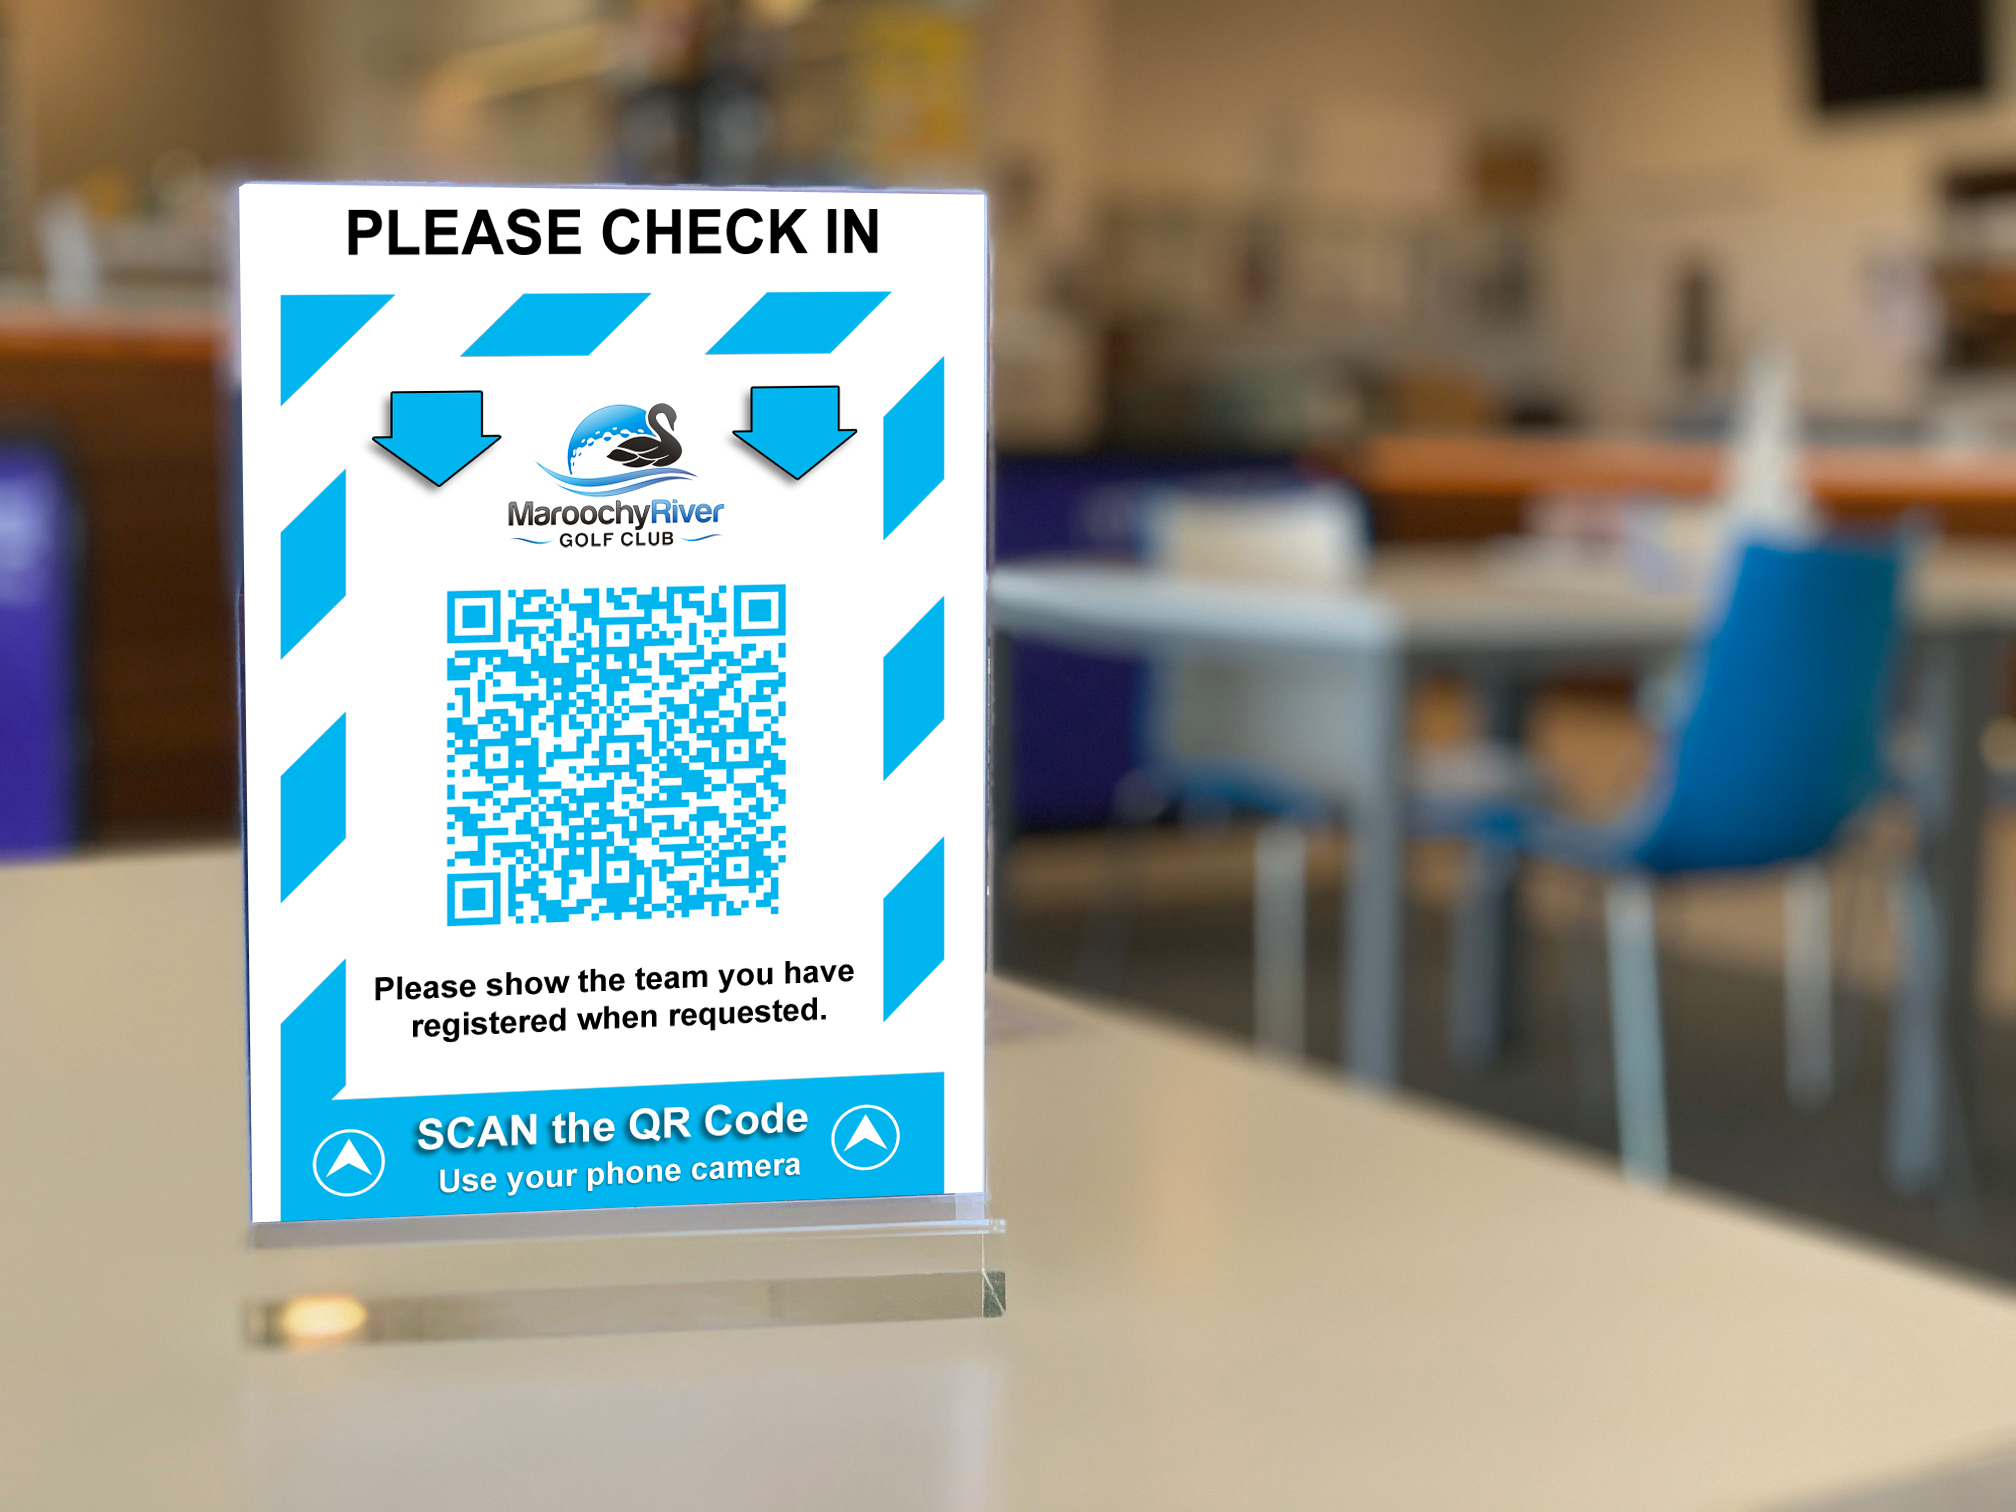
\includegraphics[width=0.3\linewidth]{qr-code-checkin.jpg}
	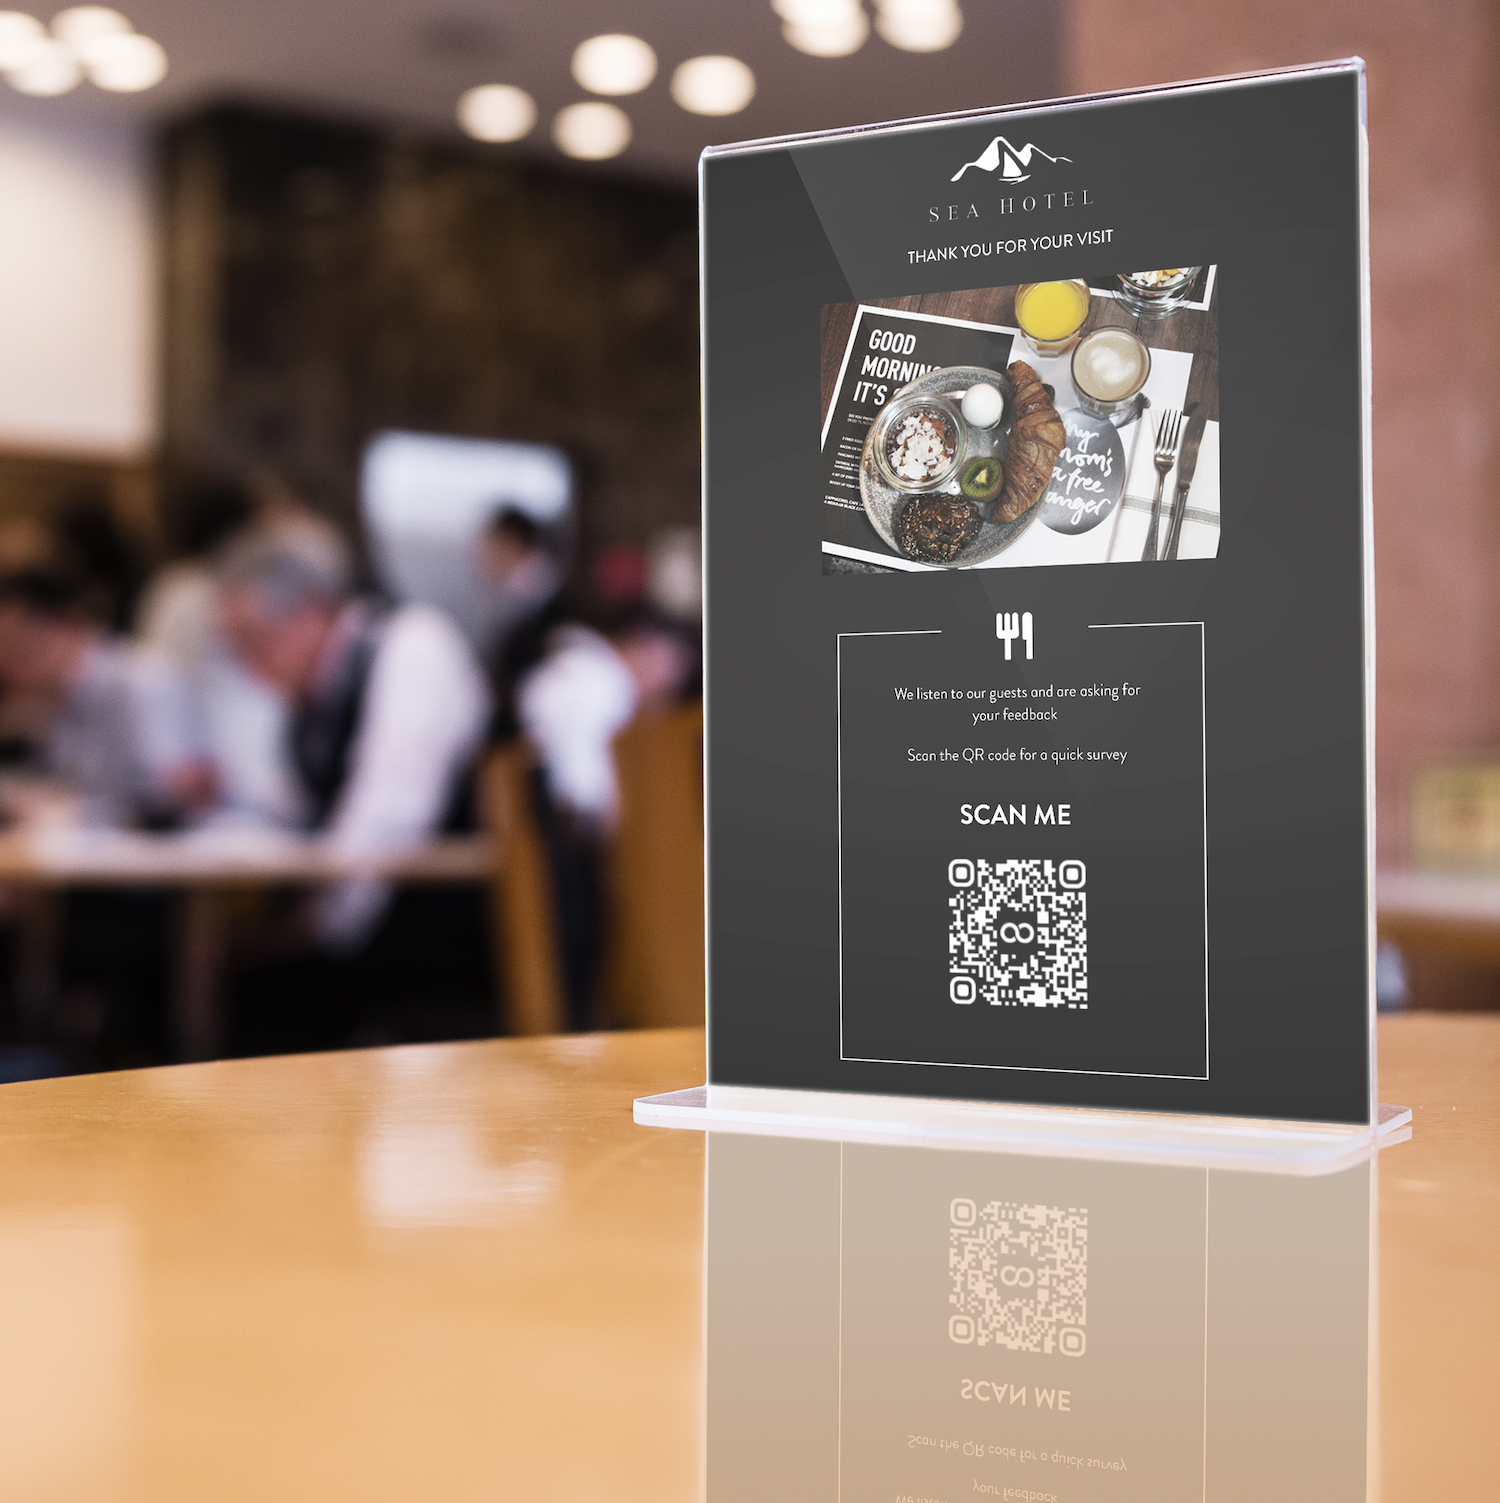
\includegraphics[width=0.3\linewidth]{qr-code-checkin2.jpg}
	\caption{El código QR en el turismo.}
	\label{fig:qrturismo}
\end{figure}

\subsection{Arquitectura y construcción}

El uso de código QR permite a las empresas de construcción y los arquitectos, a mantener los registros de capacitación de trabajadores, registros de activos y cumplir las normas de seguridad. Por ejemplo, verificar el tiempo de uso o el tiempo de vida de alguna herramienta para evitar accidentes por su deterioro en el proyecto de construcción, dado que deben seguir ciertos estándares y protocolos de calidad para garantizar la seguridad a los operadores. 
%qrconstruccion
\begin{figure} 	
	\centering
	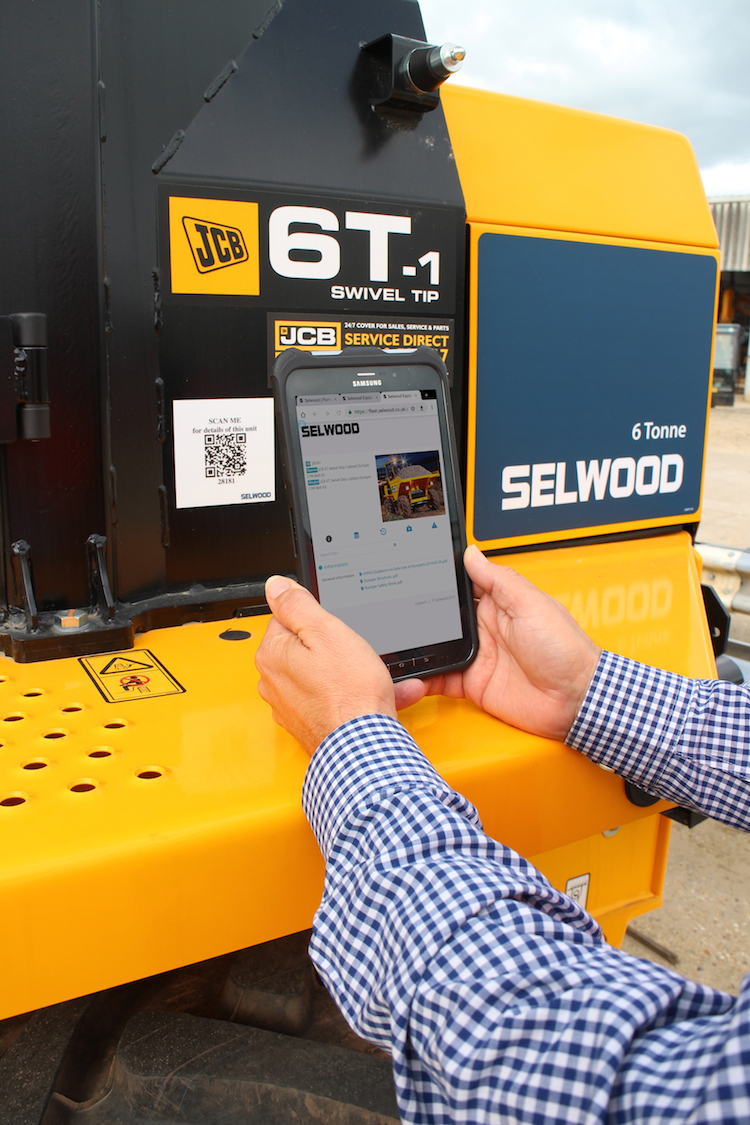
\includegraphics[width=0.2\linewidth]{qrconstruccion.jpg}
	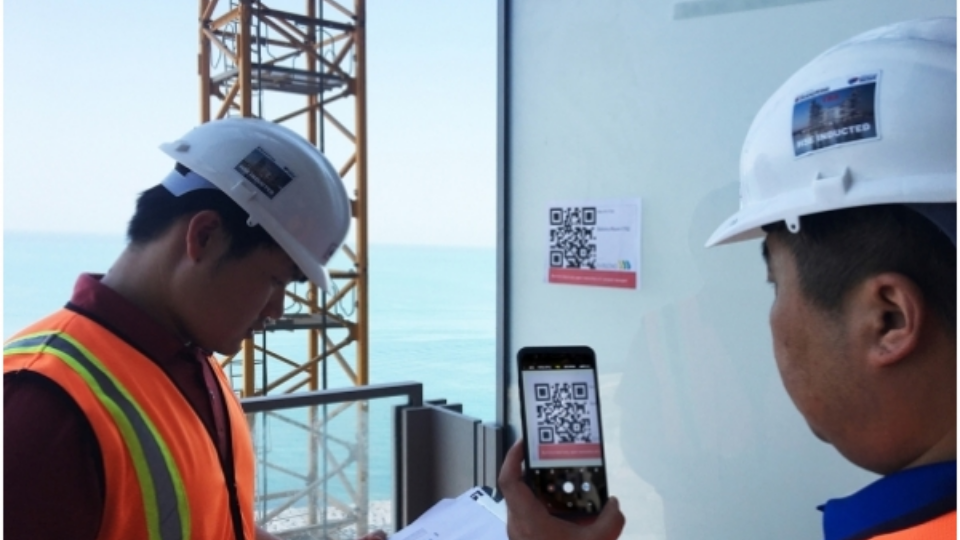
\includegraphics[width=0.4\linewidth]{qrconstruccion2.png}
	\caption{El código QR en la construcción.}
	\label{fig:qrconstruccion}
\end{figure}

El símbolo QR es utilizado para la verificación de la capacitación de los trabajadores de la construcción, para evitar lesiones, sanciones e incluso la muerte por falta de capacitación en una de las herramientas de la construcción.  Asimismo, son usados para mejorar la comprensión y simplificar el proceso de un plan de seguridad operativa o para mantenerse al día con los cambios de diseño, horarios, para evitar robos de herramientas, entre otros. \cite{delivr2021}

\subsection{Educación}
En la educación, se propuso un sistema que se ocupa de la gestión y evaluación de la asistencia de estudiantes. Donde una aplicación genera el código QR ingresando los datos del estudiante y la segunda para tomar la asistencia y generarla en formato CSV o XLS. El profesor escanea el código QR del estudiante para confirmar su asistencia, verificando la identidad del estudiante para eliminar registro falso. \cite{2017_Wei}
\begin{figure} 	
	\centering
	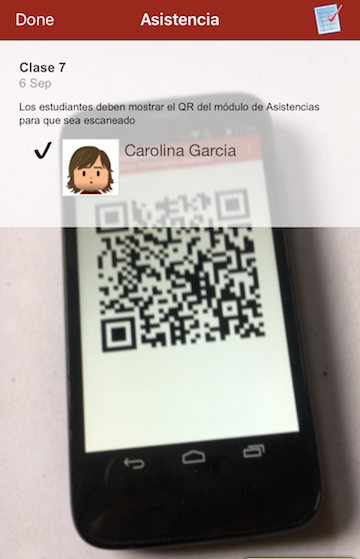
\includegraphics[width=0.2\linewidth]{asistenciaqr.png}
	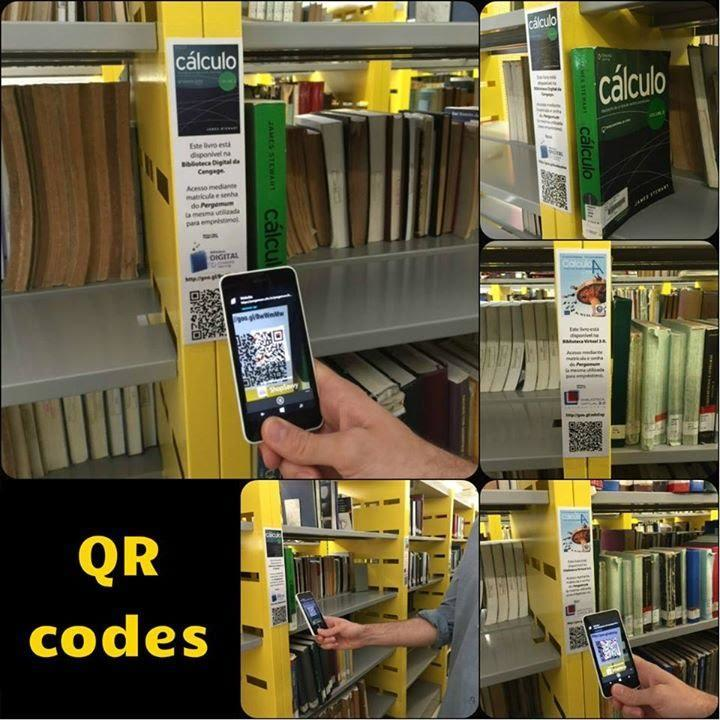
\includegraphics[width=0.3\linewidth]{qrbiblioteca.png}
	\caption{El código QR en la Educación .}
	\label{fig:qreducacion}
\end{figure}
\\
En cambio, la bibliotecas es un medio para comunicar a los usuarios sus documentos/información que desean. En el siglo XXI están completamente automatizadas, la tecnología como el código QR exige cambios en el manejo de la información en la biblioteca. El usuario mediante el uso del código QR, podra obtener información como el registro bibliográfico, añadir información básica del libro y su localización en la biblioteca.\cite{2017_Parabhoi}

\subsection{Gastronomia}
Los restaurantes utilizando la tecnología QR brindan a sus clientes información sobre el menú, la comida y bebida que se sirven, incluyendo información calórica o publicidad de porque deberian elegir su producto con respecto a la competencia. Algunos anuncios fuera del local gastronomico, podrian ofrecer descuentos en la comida o algún producto gratuito con su comida; solo para los clientes que han escaneado el símbolo QR.\cite{2012_Emek}
\begin{figure} 	
	\centering
	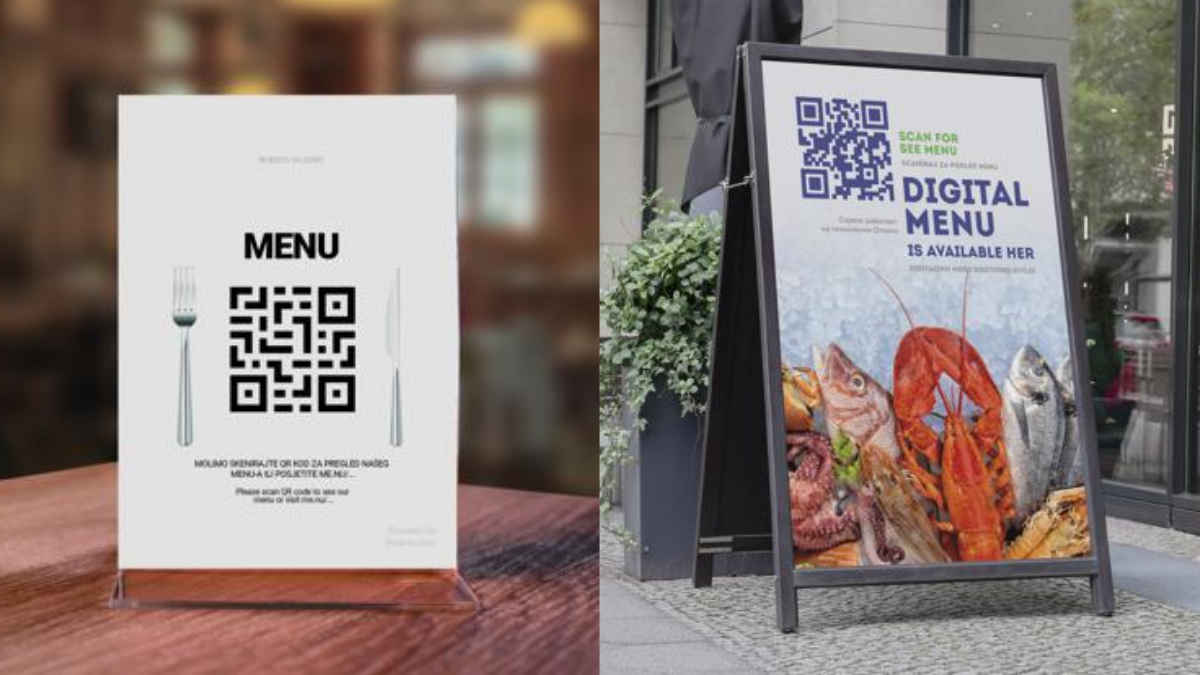
\includegraphics[width=0.6\linewidth]{qrmenu.jpg}
	\caption{El código QR en la Gastronomia .}
	\label{fig:qrmenu}
\end{figure}

\subsection{Comercio o Logística}
Con los avances en el comercio electrónico, la industria de logística no cambia mucho del transporte tradicional de mercancias, las características de lotes pequeños, velocidad y bajo costo. Al mismo tiempo, se utilizan pequeños robots como tecnología de almacenamiento flexible, ver figura (\ref{fig:datamatrixaplicaciones}). Por ejemplo, el modelo de almacenamiento flexible basado en RFID y código QR a partir del análisis de la logística. El robot planifica la ruta con estas dos tecnologías, considerando el tiempo y el conflicto de tráfico y el espacio del almacén.\cite{XiaoLong2017}
\\
Es posible realizar compras y pago por medio del escaneado del código QR, el cliente almacena sus producto en el carrito, y luego realiza el pago. \cite{2018_Banu}

\subsection{Bitcoin y Misterio-Conspiración}

El código QR es utilizado para realizar pagos con bitcoins, el símbolo contiene la ``dirección bitcoin'', que es como una dirección de correo electrónico compuesto de una larga cadenas de letras y números. Por esta razón, es utilizado para dar fácilmente su dirección a otras personas sin que tengan que escribir la larga cadena.\cite{2015_Antonopoulos_BOOK}
\begin{figure} 	
	\centering
	\includegraphics[width=0.2\linewidth]{bitcoinQR.png}
	\includegraphics[width=0.5\linewidth]{Cryptocurrency-transfer-or-payment-process.png}	
	\caption{Uso del código QR, en un proceso de transferencia y pago de bitcoins.}
	\label{fig:qrbitcoin}
\end{figure}
\\
El 4 de enero de 2012, aparecio en los foros /b/- Random Board de 4chan una imagen que fue posteada por 3301, diciendo que la imagen tenía un mensaje oculto, dando comienzo a uno de los mas grandes scavengers hunt que internet hubiera tenido, a tan solo unos minutos desde que se posteo la imagen, alguien descubrio lo que la imagen contenía, adentro tenía un string leíble  y utilizando un método de descifrado, daba una dirección web que nos dirigía a otra imagen. Luego de varios desafío de la misma forma... Se llegó que la primera imagen multiplicando su altura x ancho x 3301 = 845145127, utilizando como una dirección web: www.845145127.com, la página  web tenía un contador que al finalizar mostraba unas ubicaciones conformadas con latitud y longitud alrededor del mundo, en donde cada una de las ubicaciones tenia un código QR especial, el código almacenaba una dirección web,  que te dirigía a una imagen y está imagen tenia un acertijo, y el acertijo te llevaba a un libro y el libro te llevaba a una página donde solo un limite de personas podían ingresar, luego la página web final se quedaba fuera de servicio. \cite{lemmino2018}
\begin{figure} 	
	%\centering
	\includegraphics[width=0.9\linewidth]{cicada3301QRcodeLocations.jpg}
	\includegraphics[width=0.9\linewidth]{cicada3301QRcode.jpg}	
	\caption{Ubicación de los Códigos QRs de cicada3301 }
	\label{fig:qrcicada3301}
\end{figure}

 % Aplicaciones del código QR.

%competidores
\section{Tecnologías competidoras}

\subsection{Radio Frequency Identification - RFID}
RFID o identificación por radiofrecuencia en español, un término que describe a un dispositivo electrónico que utiliza radiofrecuencia o variaciones de campo magnético para comunicarse; que es puesto a un artículo. Los dos componentes de un sistema RFID son la etiqueta, que es el dispositivo que identifica al artículo que queremos ubicar, y el lector, que reconoce la presencia de las etiquetas,  con el fin de leer la información almacenada en ellas.
El lector obtiene la información de los elementos presentes etiquetados e informa a otro sistema de ello, siendo esta un software que se interpone entre los lectores y las aplicaciones;  middleware RFID. \cite{2006_BillGlover_BOOK}
\begin{figure} 	
	\centering
	\includegraphics[width=0.7\linewidth]{funcarfid.png}
	\caption{Tecnología RFID.}
	\label{fig:rfid}
\end{figure}
\\
RFID se está convirtiendo en una tecnología rentable, capaz de recibir y transmitir varios metros la información.\cite{2011_Coskun_BOOK} El sistema se compone de tres componentes básicos: una etiqueta en el artículo, un lector y una computadora host, vea la figura (\ref{fig:rfid}).  Las etiquetas son pequeños chips semiconductores y con antenas miniaturizadas dentro de algún tipo de empaque. Se puede rastrear e identificar a objetos o personas de forma inalámbrica por el par lector / host. \cite{2006_BillGlover_BOOK}
Por lo general, la etiqueta lee su memoria interna de datos y lo intercambia con la antena (lector), de forma codificada transmitiendo los datos.\cite{2005_Landt}
\\
El RFID aumenta la productividad y la comodidad. Utilizado para comunicar información digital entre diferentes espacios físicos y un objeto en móvil o entre objetos en movimiento. Para transferir de la etiqueta al lector utiliza el principio de retrodispersión modulada -fenomeno físico donde las ondas inciden en un material y luego son reflejadas en el mismo ángulo, volviendo a la fuente que las produjo -. \cite{2005_Landt}
\\
Esta tecnología ofrece beneficios para la gestión de la cadena de suministro, el control de inventario y suministro, gestión de la seguridad (identificación, ubicación, seguimiento y supervisión de personas y/o objetos), transporte y distribución: camiones, almacenes, etiquetas de peaje de carreteras y gestión de flotas, seguimiento de contenedores, entre otras.\cite{2007_Hunt_BOOK,2005_Weinstein}

\begin{figure} 	
	\includegraphics[width=0.5\linewidth]{lectorRFID.jpg}
	\includegraphics[width=0.5\linewidth]{tagRFID.jpg}
	\caption{Lector RFID y tipos de etiquetas.}
	\label{fig:rfid2}
\end{figure}

\textbf{Ventajas}: Alineación no es necesaria; un escaneo no requiere línea de visión, dado que es posible escanear varios artículos al mismo tiempo. Variedad de factores de forma; las etiquetas varían en tamaño. Seguimiento a nivel de artículo; identificación de forma única entre millones. Además, es posible la reescritura en algunas etiquetas, como también de una sola escritura. Transmisión de datos de corto y largo alcance. No requiere alimentación eléctrica interna las etiquetas pasivas, pero si las activas.\cite{2006_BillGlover_BOOK,2011_Coskun_BOOK}
\\
\textbf{Desventajas}: Solo para ubicar objetos y personas, no útil para pagos. Es necesario la compra del lector y el software.\cite{2005_Landt} Precio de las etiquetas dependendiendo del rango de lectura, baterías para las etiquetas activas.

\subsection{Near-Field Communication - NFC}
NFC o Comunicación de campo cercano en español, es una tecnología de comunicación inalámbrica entre dos dispositivos equipados con NFC, con una alta frecuencia de 13,56 Mhz utilizada originalmente por RFID, bajo ancho de banda y de corto alcance. La mayoría de los teléfonos móviles tienen incorporados esta tecnología, permitiendo la comunicación entre un teléfono móvil en un extremo y/o un lector NFC o una etiqueta NFC en el otro extremo.
La tecnología NFC permite el pago electrónico, emisión de billetes electrónicos, sevicios de fidelización, identificación, control de acceso, distribución de contenido, publicidad inteligente, transferencia de datos/dinero y otros servicios. \cite{2011_Coskun_BOOK}
\begin{figure} 	
	\centering
	\includegraphics[width=0.4\linewidth]{nfc1.jpg}
	\includegraphics[width=0.7\linewidth]{nfc-mode-operations.jpg}
	\caption{Tecnología NFC entre dos telefónos móviles y sus modos de operación.}
	\label{fig:nfc}
\end{figure}
\\
La comunicación de campo cercano implica dos chips NFC, cuando uno de los dispositivos se coloca cerca del chip o telefóno móvil puede solicitar al dispositivo realizar una acción específica. Por ejemplo, abrir una página web, marcar un número telefóno, compartir imagen o video, entre otros.\cite{2012_Waters_BOOK}
\\
La tecnología necesita siempre dos dispositivos, un iniciador; que genera activamente una señal de RF controlando el intercambio de datos donde la solicitud es respondida por un objetivo pásivo (móvil). Existen dos modos de comunicación: activo y pasivo. Activos donde ambos dispositivos generan sus propios campos eléctricos, lo hacen semidúplex; desactivando su campo de RF hasta que ningún otro dispositivo transmita. Ambos dispositivos suelen tener fuentes de alimentación. En cambio, el modo pasivo; solo uno genera el campo, donde el dispositivo de destino responde a esa llamada, estando en escucha y luego procesa la transferencia de datos.\cite{2012_Curran}
\\
\textbf{Ventajas}: Simple de usar; sin escaneo o sostener su teléfono, ni siquiera golpear físicamente los dispositivos, intercambio de datos seguro inherente debido a la comunicación de corto alcance, Emparejamiento implícito de parejas de parejas expresando su voluntad al realizar la comunicación. Modos de funcionamiento: reader/writer, peer-to-peer, and card emulation.\cite{2011_Coskun_BOOK}
\\
\textbf{Desventajas}: Comunicación de corto alcance, limitado a una distancia entre los dos dispositivos de hasta 10 cm.\cite{2012_Curran} Comparando con el QR es necesario comprar etiquetas de un costo no tan elevado y es necesario que el móvil tenga incorporado la tecnología.\cite{2011_Coskun_BOOK} Consumo prolongado de la batería del móvil.\cite{2012_Waters_BOOK} 

\subsection{Bluetooth Beacons}
BLE beacons o balizas BLE en español, son balizas con pequeños transmisores de radio, que se comunican a través de Bluetooth Low Energy. Las balizas son colocados en ubicaciones de forma estratégicamente para que se transmitan las señales de Bluetooth de baja energía en un rango determinado (depende del hardware).  A través de canales de BLE, se envían un número de identificación, 10 veces por segundo, donde un dispositivo con bluetooth en las cercanias de la baliza los recoge, este número es capaz de desencadenar una acción específica relevante para la ubicación (descargar una aplicación o contenido). \cite{Adarsh2021} 
\begin{figure} 	
	%\centering
	\includegraphics[width=0.4\linewidth]{beacon1.jpg}
	\includegraphics[width=0.6\linewidth]{beacon2.jpg}
	\caption{Tecnología Beacons BLE.}
	\label{fig:beacons}
\end{figure}

Esta tecnología tiene aplicaciones en el manejo de problemas de colocación o gestión de inventario, dado que el posicionamiento de los artículos es cambiante entre entregas. \cite{Octaviani2020} También son usados como marketing por proximidad, registro hiperlocal; ubicar a los visitantes con precisión, anuncios de reorientación, seguimiento de activos; las etiquetas pueden estar compuestas con sensores (luz, sonido, temperatura) que permiten el seguimiento de otros objetos y por último, navegación en interiores; marca los lugares importantes e indica la ruta recomendada. \cite{Adarsh2021}
\\
\textbf{Ventajas}: Transmisión de datos a 80 metros y también permite que el dispositivo móvil determine su ubicación siendo anónimo.\cite{Adarsh2021,Chawathe2008} 
\\
\textbf{Desventajas}: La propagación de la señal en entornos interiores es compleja y se ve afectada por muchos factores, interferencia de otros dispositivos, entre otros. El área de ubicación tiene un modelo simple como un elipsoide.\cite{Chawathe2008} El costo de la batería y de la tecnología Beacon BLE.

\subsection{Augmented reality (AR)}
La realidad aumentada superpone el mundo real con contenido digital, a través de un dispositivo tecnológico con información virtual generada por este. Es una vista en vivo, de forma directa o indirecta, del espacio físico real cuyos elementos son aumentados por algún medio audiovisual que son generados por el dispositivo. Por ejemplo, pueden permitir ver el interior de un edificio desde la acera, usando sus teléfono móviles. Alineando la pantalla del teléfono con el edificio, viendo como el mundo real es superpuesto por imagenes, videos, sonido, entre otros.\cite{2011BOOK,2012_Waters_BOOK}
%arItems
\begin{figure} 	
	\centering
	\includegraphics[width=0.5\linewidth]{arItems.jpg}
	\includegraphics[width=0.5\linewidth]{arconqr.png}
	\includegraphics[width=0.5\linewidth]{Augmented-reality-examples-_-Auto-_-Jaguar-Land-Rover-_-Blippar-carousel.jpg}
	\includegraphics[width=0.3\linewidth]{Augmented-reality-in-retail-_-Blippar.jpg}
	\caption{Tecnología de Realidad Aumentada.}
	\label{fig:ar}
\end{figure}
La tecnología tiene aplicaciones como Fig.(\ref{fig:ar}),  un sistema de navegación de interior interactivo, y el uso de la tecnología de realidad aumentada para superporner señales de dirección.También en el área de salud; estudio del corazón humano, anatomía del cuerpo humano, entre otros.	En el comercio, ayuda a mejorar la experiencia de los clientes, mostrando detalles o información del artículo (precio, nombre, modo de uso, entre otros). \cite{2021_Ong_THESIS,2021_Romli,2021_Fernandes} 
\\
\textbf{Ventajas}: el usuario puede experimentar el objeto virtual con más detalle desde varios ángulos, con lo cuál facilita mayor información y agiliza las tareas. \cite{2021_Romli}
\\
\textbf{Desventajas}: es necesario que el software sea compatible con la tecnologia AR, precio del software de realidad aumentada, dificultad de interacción con el usuario (Interfaz gráfica), requiere más tiempo de uso, problemas técnicos dados por el teléfono móvil.\cite{2018_Gavilanes}

\subsection{Image Recognition}

El reconocimiento de imágenes, es un conjunto de técnicas para identificar y analizar imágenes permitiendo la automatización de una tarea específica. Es capaz de reconocer lugares, objetos, personas y otro tipos de elementos que estan dentro de una imagen, sacando conclusiones para la toma de decisiones. Es una subcategoría de visión por computadora e inteligencia artificial, basado principalmente en Deep Learning, subcategoría de Machine Learning (uso de una red neuronal artificial entrenada mediante un conjunto de datos anotados).\cite{deepomatic.com2021,Wu2015}

\begin{figure} 	
	%\centering
	\includegraphics[width=0.5\linewidth]{imagerecognition.jpg}
	\includegraphics[width=0.5\linewidth]{teslaautopilot.png}
	\caption{Tecnología de Reconocimiento de imagen.}
	\label{fig:Irecog}
\end{figure}

Por ejemplo, el etiquetado de una imagen, ubicar algún objeto principal de una imagen o el guiado de un automóvil autónomo.
Dentro de ella tenemos, clasficación de imágenes; identificar la categoría a la que pertenece una imagen, detección de objetos; ubicar el elemento en la imagen -con un cuadro delimitador- Fig.(\ref{fig:Irecog}) , segmentación; detección de un elemento con precisión de pixel para automóviles autónomos, etiquetado; asignación de una o más etiquetas a una imagen en particular.  \cite{deepomatic.com2021}
\\
\textbf{Ventajas}: Puede reconocer cualquier elemento dentro de la imagen, incluso códigos QR u otros tipos. Solo es necesario la aplicación, una foto con su cámara o cualquier imagen y con la conexión a Internet, se obtiene resultados o contenido relacionado. \cite{lens.google2021}
\\
\textbf{Desventajas}: El reconocimiento de imagen debe estar entrenada (Hardware y Software). \cite{deepomatic.com2021,Wu2015} 

\subsubsection{Bixby Vision}
Bixby Vision es un asistente virtual disponible en teléfonos móviles samsungs, las funciones disponibles son: traducción de texto de un idioma a otra en la vista previa en vivo de la pantalla, permite realizar búsquedas de imagenes similares a la imagen tomada con la cámara, con ello podemos realizar una búsqueda de artículos similares. Lectura de un código QR, descriptor de escena, identificador de objetos, lector de texto desde una imagen, entre otros. \cite{samsung.com2021}
\begin{figure} 	
	%\centering
	\includegraphics[width=0.5\linewidth]{bixby1.jpg}
	\includegraphics[width=0.5\linewidth]{bixby3.jpg}
	\caption{Bixby Vision, Reconocimiento de imagenes.}
	\label{fig:Irecog2}
\end{figure}

\subsubsection{Google Lens}
Google lens es una aplicación móvil de reconocimiento de imagen diseñada para mostrar información, a partir del análisis de una imagen, generando varios resultados posibles y clasificarlos según la relevancia. Por ejemplo, si una imagen incluye un producto específico (ropas o jeans), puede mostrar resultados que brinden más información sobre el producto o que ofrezcan opciones para comprarlo. Puede utilizar códigos de barras o texto en una imagen, con esto puede mostrar una página de resultados. Tiene varias funciones: comprender lo que se está mirando, traducir texto o copiar, identificar algún animal o objeto, explorar lugares o menús, descubrir productos, entre otros.\cite{lens.google2021}
\begin{figure} 	
	%\centering
	\includegraphics[width=0.5\linewidth]{Google-Lens-1.jpg}
	\includegraphics[width=0.5\linewidth]{Google-Lens-2.jpg}
	\caption{Google Lens, Reconocimiento de imagenes.}
	\label{fig:Irecog3}
\end{figure}


\subsection{LinkRay Light ID}

LinkRay es una tecnología de que permite transmitir información a un teléfono móvil que cuenta con la aplicación, a través de la luz led visible, por medio de los letreros LED y pantallas LED, entre otros. También son usadas en la comunicación, en el marketing, industrias de turismo, venta minorista, hotelería, transporte y gestión de eventos. Por ejemplo, informar las condiciones del tráfico en tiempo real, ofrecer cupones en comercios, publicidad dirigida a usuarios optativos como forma de aumento de las ventas y el servicio.
A partir de la luz que emiten los transmisores LED, es posible leer las etiquetas identificativas. Los datos enviados al usuario pueden ser archivos de imagen, audio o vídeo. \cite{Business2017}
\\
\textbf{Ventajas}: Velocidad de transmisión por medio de la luz led visible.\cite{Business2017}
\\
\textbf{Desventajas}: En desarrollo desde su presentación en 2017\cite{Business2017}

\begin{figure} 	
	%\centering
	\includegraphics[width=0.5\linewidth]{linkray_system_configuration_1.png}
	\includegraphics[width=0.4\linewidth]{LinKRayGraphs.png}
	\includegraphics[width=0.4\linewidth]{Panasonic-Light-ID.jpg}
	\includegraphics[width=0.5\linewidth]{linkrayMuseum.jpg}
	\caption{Tecnología LinkRay Light ID.}
	\label{fig:linkray}
\end{figure}


 % Tecnologías que compiten con el código QR.

%conclusion 
\section{Conclusión}
Para concluir, el código QR es la evolución del código de barras unidimensional, dado que combina escaneo rápido, adaptación al tamaño de los datos, resistencia a errores y daños, alta capacidad de almacenamiento tanto en su dimensión horizontal y vertical. Siendo uno de los métodos para transferir información, no solo para el sector industrial sino también para otras. Esta tecnología se encuentra en la mayoria de los productos de consumo y va apareciendo con más fuerza en otras áreas aumentando la automatización.
\\
Desde su introducción, ha sido un método de entrada, preciso, rápido y con bajo coste en su forma impresa. Los tipos de códigos QR disponibles, permiten gran variedad de aplicaciones en la vida diaria.  Además, las variantes de los códigos bidimensionales muestran las grandes distinciones en su uso y aplicabilidad en determinados sectores, como algunos destacan por su velocidad de lectura sin importar si se encuentran en movimiento, capacidad de codificación, su tamaño mínimo, demostrando que cada uno ofrece algo diferente para un determinado fin.
\\
Sin duda alguna, el símbolo QR se encuentra en muchas áreas algunas son: medicina, marketing y publicidad, entretenimiento, arquitectura y construcción, educación, gastronomia, comercio , entre otros. Cada una de las cuales las utiliza con un propósito diferente, con la capacidad de ofrecer otras formas no ideadas hasta el momento. Sobre todo con el aumento de dispositivos móviles, intentando acelerar su adopción mediante el marketing o el uso en industrias automatizadas.
\\
Sin embargo, si bien existen otras tecnologías capaz de optimizar los tiempos de lectura, con mayor cantidad de modos de funcionamiento, con mayor longitud en cuanto a la transmisión de datos, con mejores presentaciones, y con nuevas mejoras que el código QR no cuenta. A pesar de ello, el código QR permite complementarse con otras tecnologías sin mucha dificultad, siendo ésta en realidad una de sus mejores características.
\\
Finalmente, el código QR necesita una razón que fundamenta porque debería ser escaneada. Un ejemplo de esto sería el uso en la gastronomia, el símbolo es usado para remplazar la pancarta del menú. Actualmente son usados para intercambiar números de telefónos o nombres de usuarios en redes sociales, sin la necesidad de buscarlos en un buscador. %Conclusion del trabajo

% Bibliografias
\bibliographystyle{unsrt} 
%\bibliographystyle{splncs04} % Falla, da un formato raro a las URLs -Deja sin margenes.-
\bibliography{./QR_Bib} % Archivo .bib


\end{document} % Final del cuerpo del documento. (Cierre) Todo posterior a esta será ignorado por LATEX y no se compilará.-------------------